% !TeX root = ./Document.tex
\documentclass[12pt,a4paper]{report}

\newcommand{\Author}{Cornelius Scheepers}
\newcommand{\AuthorTitle}{Mr}
\newcommand{\ThesisTitle}{Using user-based activity logging and analysis to prioritise software maintenance}
\newcommand{\DegreeName}{Master of Engineering in Computer and Electronic Engineering}

\newcommand{\FooterTitle}{\ThesisTitle}%\ - \Author}
\newcommand{\Supervisor}{Dr Jaco Prinsloo}
\newcommand{\FinalDate}{\today}
\newcommand{\StudentNumber}{25899880}
\author{\Author}
\title{\ThesisTitle}

\newcommand{\ChapterPageStuff}[1] {
    \begin{center}
    \vspace{2mm}
    
\includegraphics[height=15cm]{src/includes/ChapterFiles/chapter#1/figures/chapter.pdf}
    \end{center}
    \vfill
    \begin{center}
    \footnotesize
    \hrule
    \vspace{5mm}
    \ThesisTitle\\\Author
    \normalsize
    \end{center}
    \pagebreak
}
\newcommand{\etal}{\textit{et~al.}}

% Include other packages
\usepackage[hidelinks]{hyperref}
\usepackage{cite}
\usepackage{graphicx}
\usepackage{float}
\usepackage{multirow}
\usepackage{array, tabularx}
\usepackage{xltabular}
\usepackage[hang]{footmisc}
\setlength\footnotemargin{10pt}
\usepackage[font=footnotesize,skip=4pt]{caption}
\usepackage{cleveref}
\usepackage{textcomp}
\usepackage{pdfpages}
\usepackage{cprotect}
\usepackage{ragged2e}
\usepackage{pifont}
\usepackage{pdflscape}
\usepackage{enumitem}
\usepackage{tcolorbox}
\usepackage{booktabs}
\usepackage{makecell}
\usepackage{threeparttable}
\usepackage{colortbl}
\usepackage{xcolor}
\usepackage{orcidlink}
\usepackage{comment}
\usepackage{setspace}
\newenvironment{notes}
    {\color{rednotes} \begin{footnotesize}} {\color{black}\end{footnotesize}}

\definecolor{lightgray}{rgb}{.95,.95,.95}
\definecolor{darkgray}{rgb}{.4,.4,.4}
\definecolor{purple}{rgb}{0.65, 0.12, 0.82}
\definecolor{deepblue}{RGB}{0,0,128}
\definecolor{pastelgreen}{RGB}{152,251,152}

% Check mark and cross
\newcommand{\cmark}{\ding{51}}
\newcommand{\xmark}{\ding{56}}
\crefrangeformat{equation}{Equations~(#3#1#4--#5#2#6)}
   
% Prepare TOC
\usepackage{tocloft}
\renewcommand{\contentsname}{Table of contents}
\setcounter{tocdepth}{1}
\renewcommand{\cftchapleader}{\cftdotfill{\cftdotsep}} % for chapters
\usepackage[parfill]{parskip}

%% Alternative chapter styling - also remove \ChapterPageStuff \usepackage{etoolbox}
%\patchcmd{\chapter}{\thispagestyle{plain}}{\thispagestyle{fancyfooter}}{}{} Define chapter heading
%formats and spacing
\usepackage{titlesec}
\titleformat{\chapter}[display] {\normalfont\huge\bfseries} {\chaptertitlename\ \thechapter} {20pt}
  {\Huge} [\vspace{1ex}\titlerule]
\titlespacing*{\chapter}{0pt}{0pt}{40pt}
\renewcommand{\cftaftertoctitle}{\vspace{5mm}\hrule}

% Define page layout
\usepackage[bindingoffset=0.5cm, top=2.5cm, bottom=2.5cm, left=2cm, right=2cm]{geometry}

% Define header and footer layout for first pages
\usepackage{fancyhdr}
\pagestyle{fancy}
\fancyhead{}

% List words that should not be hyphenated
\hyphenation{Eskom}
\graphicspath{{img/}}

\hypersetup
{pdfauthor={\Author}, pdftitle={\ThesisTitle}, pdfcreator={\Author}, pdfkeywords={Software
    maintenance, event logging, logging mechanisms, user activities,data-driven decision-making,
    system utilisation analysis, Web-based}}

\usepackage{listings}
\crefname{lstlisting}{listing}{listings}
\Crefname{lstlisting}{Listing}{Listings}

%\setlength{\tabcolsep}{10pt} % Default value: 6pt
\renewcommand{\arraystretch}{1.5} % Default value: 1

\newcommand\JSONnumbervaluestyle{\color{blue}}
\newcommand\JSONstringvaluestyle{\color{red}}
\newcolumntype{Y}{>{\centering\arraybackslash}X}
\newcolumntype{P}{>{\raggedleft\arraybackslash}X}

% Continue table text
\newcommand{\continueCaption}{\textit{(continued from previous page)}}
\newcommand{\continueText}{\scriptsize Continued on next page}

% switch used as a state variable
\newif\ifcolonfoundonthisline

\makeatletter

\lstdefinestyle{json}
{
  showstringspaces    = false,
  keywords            = {false,true},
  alsoletter          = 0123456789.,
  morestring          = [s]{"}{"},
  stringstyle         = \ifcolonfoundonthisline\JSONstringvaluestyle\fi,
  MoreSelectCharTable =%
    \lst@DefSaveDef{`:}\colon@json{\processColon@json},
  basicstyle          = \ttfamily,
  keywordstyle        = \ttfamily\bfseries,
  frame=trbl,
  frameround=tttt,
  framesep=4pt,
}

\lstdefinelanguage{JavaScript}{
  keywords={typeof, new, true, false, catch, function, return, null, catch, switch, var, if, in, while, do, else, case, break},
  keywordstyle=\color{blue}\bfseries,
  ndkeywords={class, export, boolean, throw, implements, import, this},
  ndkeywordstyle=\color{darkgray}\bfseries,
  identifierstyle=\color{black},
  sensitive=false,
  comment=[l]{//},
  morecomment=[s]{/*}{*/},
  commentstyle=\color{purple}\ttfamily,
  stringstyle=\color{red}\ttfamily,
  morestring=[b]',
  morestring=[b]"
}

\lstset{
   language=JavaScript,
   backgroundcolor=\color{lightgray},
   extendedchars=true,
   basicstyle=\footnotesize\ttfamily,
   showstringspaces=false,
   showspaces=false,
   numbers=left,
   numberstyle=\footnotesize,
   numbersep=9pt,
   tabsize=2,
   breaklines=true,
   showtabs=false,
   captionpos=b
}

% flip the switch if a colon is found in Pmode
\newcommand\processColon@json{%
  \colon@json%
  \ifnum\lst@mode=\lst@Pmode%
    \global\colonfoundonthislinetrue%
  \fi
}

\lst@AddToHook{Output}{%
  \ifcolonfoundonthisline%
    \ifnum\lst@mode=\lst@Pmode%
      \def\lst@thestyle{\JSONnumbervaluestyle}%
    \fi
  \fi
  %override by keyword style if a keyword is detected!
  \lsthk@DetectKeywords% 
}

% reset the switch at the end of line
\lst@AddToHook{EOL}%
  {\global\colonfoundonthislinefalse}

\makeatother

% counters
\newcounter{phase}
\renewcommand*{\thephase}{F/R~\arabic{phase}}

\newcounter{subphase}[phase]
\renewcommand*{\thesubphase}{\thephase.\arabic{subphase}}

\newcounter{subsubphase}[subphase]
\renewcommand*{\thesubsubphase}{\thesubphase.\arabic{subsubphase}}

\newcommand*{\phase}[1]{%
  \leavevmode
  \refstepcounter{phase}%
  \label{#1}%
  \thephase%
}
\newcommand*{\subphase}[1]{%
  \leavevmode
  \refstepcounter{subphase}%
  \label{#1}%
  \thesubphase%
}
\newcommand*{\subsubphase}[1]{%
  \leavevmode
  \refstepcounter{subsubphase}%
  \label{#1}%
  \thesubsubphase%
}

% ---------------------------- Start the document -------------------------------------

\begin{document}
\begin{onehalfspace}
% Set header height
\renewcommand{\headheight}{15pt}

% Generates the title page
\begin{titlepage}

\includepdf[pages=-]{src/includes/TitlePageOfficial.pdf}
\end{titlepage}

%Set page numbering for first pages
\pagenumbering{roman}

% ------- Abstract -------

\cleardoublepage
\fancyhead[R]{Abstract}
\chapter*{Abstract}
\addcontentsline{toc}{chapter}{Abstract}

\begin{tabular}{l p{12cm}}
    \textbf{Title:} & \ThesisTitle\\
    \textbf{Author:} & \AuthorTitle\ \Author\\
    \textbf{Supervisor:} & \Supervisor\\
    \textbf{Degree:} & \DegreeName\\
    \textbf{Keywords:} & maintenance, logging mechanisms, user activities, system utilisation, Web-based\\
\end{tabular}
%\vspace{24pt}
% TODO Edit Abstract

Maintenance of software is continuous and is a reduced form of software
development. Research suggest that $15\%$ of the total development cost is to
implement a maintenance model on a specific software system. Unused software
components or software not meeting the user's requirements will increase over
the life cycle of the project. Deprecating some of these systems may reduce the
amount resources needed to maintain the entire project. Deciding how much
resources for maintenance needs to allocated to each system can be difficult
without a suitable method.

Software logging is essential mechanism to improve software maintenance in the
form of troubleshooting. In large software systems logging enables the
development team to monitor specific events. System utilisation of each software
system can identified if a suitable logging mechanism is implemented. In
Web-based applications the utilisation of each software system is based on how
much the users will interact with it. The interactions between the user the
software system can be logged.

Analysing these logs can be difficult when the logging mechanism does not track
the desired user-based events. Developing a method to track these events for a
specific purpose is more efficient. Relevant data creates more effective
analysis of a specific topic and increases optimisation of a model. The need to
integrate the method used to create a logging mechanism and analysing the data
will improve the maintenance of software systems.

During this study a method is developed for a Web-based application to track the
user's activities. The logging mechanism is designed to get any user activities
on any software systems they are interacting with. Ajax-requests contains
significant and relevant data than tracking all the actions of the user of a
specific event. Capturing each Ajax-requests generated from the user activities
is the main communication interface between the user's client device and the
server that runs the software systems.

Analysis is performed on the logs that was obtained from the user activity
logging mechanism. Software systems utilisation is compared to each other. The
resources allocated to maintain each software system is compared to each other.
Using the resource allocated and the system utilisation new decisions can be
made of the software maintenance. This form part the data-driven decision making
about the utilisation of the different software components.


% ------- Acknowledgements -------
%--------------------------------------------------------------------
%                        Acknowledgements
%--------------------------------------------------------------------

\cleardoublepage
\fancyhead[R]{Acknowledgements}
\chapter*{Acknowledgements}
\addcontentsline{toc}{chapter}{Acknowledgements}

I want to express my heartfelt thanks to my parents, Albert and Mirriam Scheepers, for their unwavering support through all these years. Your love and encouragement have been my guiding light, and I couldn't have done it without you. I also want to extend my gratitude to my brothers, Tyron and Danzel, and my sister, Claudia, for always being there with me on this journey.\par I'm also deeply grateful to ETA-Operations (Pty) Ltd for granting me the opportunity to pursue my master's degree through an IPGIP-bursary under the guidance of Prof. E.H. Mathews.\par I want to extend my sincere appreciation to Dr. Jaco Prinsloo, my supervisor, and Dr. Jano de Meyer, my mentor, who helped me during my most difficult times. Your unwavering support and guidance were invaluable, and I am thankful for your mentorship.\par A special thanks also goes to my previous supervisors, Dr. Pieter Goosen and Dr. Jan Vosloo, for getting me started on my master's journey. \par I would also like to express my gratitude to Megan Lowes for her meticulous proofreading of my work and her incredible patience with me. Your assistance was invaluable in the final stages of my journey. \par Lastly, I want to thank my colleagues and friends for their support and encouragement throughout this journey. Your friendship has made this experience even more memorable and meaningful. And to Kaido, the most faithful leopard gecko.

% ------- Table of contents -------
\cleardoublepage
\fancyhead[R]{\contentsname}
\chapter*{\contentsname}
\addcontentsline{toc}{chapter}{\contentsname}
\makeatletter\@starttoc{toc}\makeatother

% ------- List of Figures -------
\cleardoublepage
\fancyhead[R]{List of figures}
\chapter*{List of figures}
\addcontentsline{toc}{chapter}{List of figures}
\makeatletter\@starttoc{lof}\makeatother

% ------- List of Tables -------
\cleardoublepage
\fancyhead[R]{List of tables}
\chapter*{List of tables}
\addcontentsline{toc}{chapter}{List of tables}
\makeatletter\@starttoc{lot}\makeatother

% ------- Nomenclature -------

%--------------------------------------------------------------------
%                          Nomenclature
%--------------------------------------------------------------------

\cleardoublepage
\fancyhead[R]{Nomenclature}
\chapter*{Nomenclature}
\addcontentsline{toc}{chapter}{Nomenclature}

\begin{center}
Abbreviations:
\end{center}
\begin{table}[H]
\centering
\begin{small}
{\tabulinesep=1.4mm
\begin{tabu}{ | l | l | }
        \hline \textit{IEEE} & Institute of Electrical and Electronics Engineers \\
        \hline \textnumero & Ordinal numeration \\
        \hline AJAX & Asynchronous JavaScript and XML \\
        \hline
\end{tabu}}
\end{small}
\end{table}

\begin{center}
Units:
\end{center}
\begin{table}[H]
\centering
\begin{small}
{\tabulinesep=1.4mm
\begin{tabu}{| l | l | l |}
        \hline kVAr     & Kilovolt-ampere          & Reactive power\\
        \hline kW       & Kilowatt                 & Power\\
        \hline kWh      & Kilowatt-hour            & Energy\\
        \hline GW       & Gigawatt                 & Power\\
        \hline GWh      & Gigawatt-hour            & Energy\\
        \hline ML       & Megalitre                & Volume\\
        \hline MVA      & Megavolt-ampere          & Apparent power\\
        \hline MW       & Megawatt                 & Power\\
        \hline MWh      & Megawatt-hour            & Energy\\
        \hline R        & South African Rand (ZAR) & Currency\\
        \hline
\end{tabu}}
\end{small}
\end{table}


%-------------------------------------
% Fix page numbering for start of body
\pagenumbering{arabic}
\setcounter{page}{1}
% Setup header and footer for content pages
\fancyhead[R]{\leftmark}
\renewcommand{\chaptermark}[1]{\markboth{\chaptername \ \thechapter.\ #1}{}} 
\fancyfoot{} % clear all footer fields
\fancyfoot[L]{\footnotesize \FooterTitle}
\fancyfoot[R]{\thepage}%\vspace{2mm}
\renewcommand{\headrulewidth}{1.5pt}
\renewcommand{\footrulewidth}{1.5pt}

% ------- Chapters -------
\chapter{Introduction}
\label{chap:1}
\ChapterPageStuff{1}

\section{Preamble}
Maintenance of software systems is continuous and is a reduced form of software
development \cite{Sneed2004}.~Software maintenance needs to be done on regular
systematically procedure in its entire lifespan. Most companies will strife to increase their digital products and services over the life cycle of the software project \cite{Niu2018},\cite{Galster2019}.

\section{Background}
Software maintenance is an essential task in software development, it can directly reduce cost and effort to create new software systems \cite{FrancisThamburaj2017}. According to a study of the total development cost for typical software maintenance efforts, conducted by the United States Department of Commerce found that the cost can be as much as $60\%$-$80\%$ of the total cost of the software systems entire development life cycle \cite{Ogheneovo2014}, \cite{Stark1996}. These costs will increase (as in Fig.~\ref{fig:CH1_Costs_of_fixing_bugs}) to maintain much older and more complexed software systems, therefore it is key to the feasibility of the software systems to implement maintenance on it \cite{Alenezi2016}, \cite{Booch1986}.

\begin{figure}[!htb] % An h :here, t: top, b: bottom.
    \centering % cent the figure
    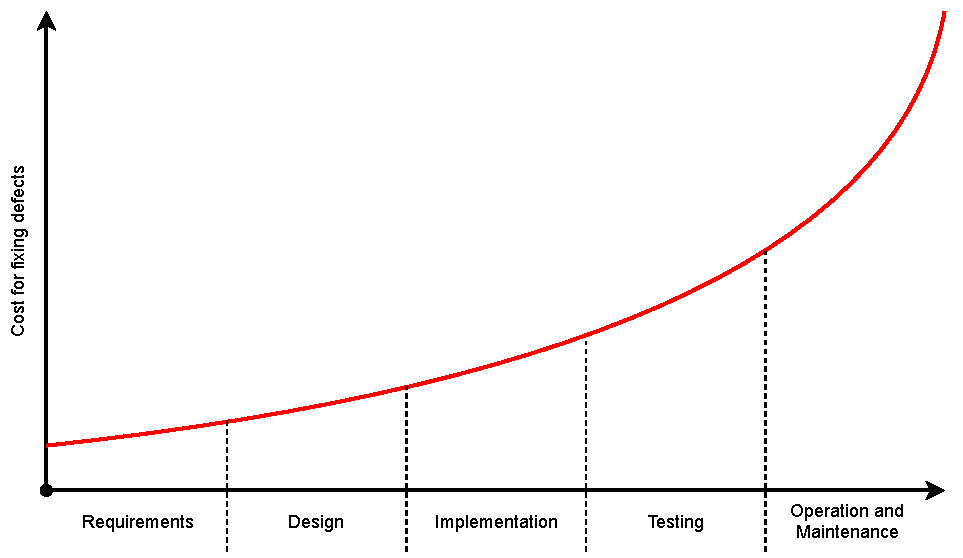
\includegraphics[width=0.7\textwidth]{Images/Chapter1/Background/Cost_of_fixing_bugs/Cost_of_fixing_bugs.pdf}
    \caption{Cost of fixing software system defects \cite{Ogheneovo2014}}\label{fig:CH1_Costs_of_fixing_bugs}
\end{figure} 

Under most circumstances maintenance is implemented if a software system does not meet the required functions specified by the performance requirements \cite{Ogheneovo2014},\cite{Sneed2004}. These systems will also most likely have multiple software defects or will be extremely complex due to:
\begin{itemize}
    \item \textbf{Problem domain being complex:} The software may not be well defined or structured. This is due how large the software systems grow over its entire life cycle or duplicate software components that are made. This is caused by poor understanding of the system architecture by developers not doing the required maintenance on these systems and just adding new features \cite{Galster2019}, \cite{Booch1986}.
    \item \textbf{Difficulties of managing development process:} Most companies will strife to increase their digital products and services over the life cycle of the software project to maximize possible profits with the resources invested \cite{Niu2018}. Increasing production of the development process will only strain the efforts of maintaining software systems \cite{Sneed2004}. The development team needs to prioritize concrete task in the development process to make the project feasible, by just focusing on these task poor decisions are made about the required task to perform software maintenance \cite{Galster2019}, \cite{Ogheneovo2014}, \cite{Lenarduzzi2017}. 
    \item \textbf{Flexibility of the software:} Trying to predict what the possible future architecture may look like and modifying it while preserving its integrity, may be difficult in software maintenance \cite{Garlan1999}. Software is flexible if it is adaptable to the problem domain when adding modifications to it \cite{Ogheneovo2014}. Most development teams will follow a 
\end{itemize}
\newpage

\subsection{Need for a logging mechanism}
No study was found where both the logging mechanism and analysis were combined.
There is a need to develop a method to implement a user-activity logging
the mechanism to do further analysis of the logs to improve software
maintenance.

\subsection{Objectives of the study}
The goal of the study is to develop a logging mechanism to track user-based
activities to preform analysis of these logs to improve system maintenance in
software environment. The study is divided in two components to achieve the
primary goal which is the design and implementation of the logging mechanism
and the analysis of the system utilisation to improve system maintenance.

\subsubsection{Logging mechanism:}
\begin{itemize}
    \item Random text.
\end{itemize}

\subsubsection{Analysis of the system utilisation to improve software maintenance}
\begin{itemize}
    \item Random text.
\end{itemize}

\subsection{Overview of the dissertation}
\subsubsection{Chapter 1: Introduction}
This chapter contains the background of software maintenance and system
utilisation analysis.
\subsubsection{Chapter 2: Mehtodolgy}

\newpage
\section{Literature Study}

\subsection{Preamble}
Introduction of section.

\subsection{Software Maintenance}

\subsection{Event-based logging}
In this section the event-based logging will be discussed and how it is part of software maintenance. 

\subsection{User-based activities in Web-based applications}
In this section, the user-activities in Web-based applications will be discussed.

\subsection{Logging mechanism development}

\section{Conclusion}


\chapter{Methodology}
\label{chap:2}
\ChapterPageStuff{2}

\section{Preamble}
In this chapter the methodology to create and implement a logging mechanism to do system utilisation analysis on software system will be discussed. In \Cref{sec:EventLogging} provided the needed literature to create a logging mechanism in \Cref{sec:Ch3_LoggingMechanism} for two software systems.

\section{Logging mechanism}\label{sec:Ch3_LoggingMechanism}
For this study two software systems are used to implement two different logging mechanisms. The first software system which will be called System A, is energy management system that uses \emph{PHP}. System B is a \emph{.NET Framework}\footnote{\label{ftn:NetFramework}\textbf{.NET Framework} is a run-time execution environment that consists of common language run-time (\emph{CLR}) and a \texttt{.NET Framework Class Library} \cite{Harkness2007}.} system with a \emph{MVC} architecture as in \Cref{fig:ch2_Flow_MVC_Architecture} and is the administrative software system to configure System A.

\subsection{System A}
Logging point are essential data that describes the event's key features when creating a log as discussed in \Cref{sec:Ch1_LoggignPoints}. Both System A and B have certain key logging points that needs to be obtained from the user generated event.

\subsubsection{System A's logging points}\label{sec:SystemA_LoggingPoints}
In \Cref{fig:ch2_SystemA_Dashboard} each mine group have multiple toolboxes linked to them. They can be same toolbox linked to both mine groups such as \emph{T1} and \emph{T3}. These toolboxes represent a group of dashboards related to the aspects of energy management of mines.\par Each of these toolboxes have a dashboards linked to them and each mine group can have different dashboards linked to the to the same toolbox. Each one of these mine groups, toolboxes and dashboards forms part of System A's web pages which the user can access where event logs are generated.

\begin{figure}[!htb] % An h :here, t: top, b: bottom.
	\centering % cent the figure
	\includegraphics[width=0.8\textwidth]{Images/Chapter2/SystemA_Dashboard/SystemA_Dashboard.pdf}
	\caption[System A dashboard links]
	{\textit{System A dashboard links}}\label{fig:ch2_SystemA_Dashboard}
\end{figure}

Each dashboard in \Cref{fig:ch2_SystemA_Dashboard} can use the same files to create the a dashboard by only configuring the content of the dashboard based on the request parameters that is send when the user navigates to a new dashboard. Capturing the user generated events with a logging mechanism can be done in these shared files instead of the entire software components of System A.\par The user session helps to keep to track of any information needed for these pages to be fully functional like the user's identity and dashboard related data. This information can be used to give insight on which page the user is currently active on. In this case for System A the important user session information is:

\begin{itemize}
	\item \textbf{User's identity:} The session contains the user's name and identity number which is the unique primary key for the user. This session information will always be available if the user is active on the software system from the instance they are logged in and verified until the user logs out and close their browser.
	\item \textbf{Group identity:} System A is used for multiple mine companies, each of the mining companies have a unique identity number. Each group have multiple toolboxes linked to them for energy management.
	\item \textbf{Dashboard identity:} Each dashboard uses certain files to construct a web page the user can view. To correctly navigate and get the correct page when the user request it, a unique identity number is used. In some cases for this system the same file can be used for multiple dashboards as extra configuration data is obtained from the database for that specific dashboard identity number.
	\item \textbf{Configuration meta data identity:} In \Cref{fig:ch2_SystemA_Dashboard} the same dashboard can be linked to different mine groups or toolboxes. The user session contains any other identification parameters of which meta data should be loaded to configure the dashboard for the correct mine group and toolbox.
\end{itemize}

\begin{table}[!htb]
	\centering
	\small
	\caption[Logging points]
	{\textit{System A user activities table}}
	\label{tbl:Ch2_System_A_Logging_Points}
	\begin{tabularx}{\textwidth}{|l|l|X|}
		\hline \textbf{Column Name} & \textbf{SQL Data Type} & \textbf{Description} \\
		\hline \textbf{ActivityID} & INT(11) & The activity identification is an incremental number of the event that is logged.\\
		\hline \textbf{Timestamp} & DATETIME & This is the time which the event took place.\\
		\hline \textbf{UserID} & INT(45) & Each user has a unique identifier which is a numerical identification number that is foreign key reference to the User table.\\
		\hline \textbf{DashboardID} & INT(4) & Foreign key reference to the Dashboard table. \\
		\hline \textbf{GroupID} & INT(4) & This foreign key reference to the Group table is contract groups identification number. \\ 		
		\hline \textbf{ActivityType} & ENUM & Each event that user initiated has an activity type as in \Cref{tbl:Ch2_SystemA_EventTypes}. \\
		\hline \textbf{File} & VARCHAR(200) & This the PHP file from which the request is processed.\\
		\hline \textbf{RequestParameters} & JSON & Request parameters of the event. This can be other meta data that is important about the user's activity using certain controls on a dashboard or toolbox. \\
		\hline
	\end{tabularx}
\end{table}

\clearpage

Obtaining the key information of the user generated event is essential to define which key logging points the logging mechanism needs to get from the user's session. In \Cref{tbl:Ch2_System_A_Logging_Points} System A's key logging points which are saved in a SQL database. Each logging point can be accessed either by the user session or other run-time data present when the event took place such as any meta data that as send back the server as request parameters.

The user activity types in \Cref{tbl:Ch2_SystemA_EventTypes} is all of the possible activities the user can generate in System A. The DetailView activities is expected to the largest portion of events that will be tracked as users will generally try to use multiple input elements on the dashboard or toolbox. \par The Dash event type is only useful to track which dashboards and toolboxes the user navigates to and it will not be accurate indicator to how much a dashboard or toolbox is used. The DetailView and Report user activity types is better representation of the utilisation of these software components as these events are the user's objectives using the software systems and not trying access the software systems.  

\begin{table}[!htb]
	\centering
	\small
	\caption[System A user activity types]
	{\textit{System A user activity types}}
	\label{tbl:Ch2_SystemA_EventTypes}
	\begin{tabularx}{\textwidth}{|l|X|}
		\hline \textbf{Activity Type} & \textbf{Description} \\
		\hline \textbf{Dash} & Any activity that the user attempts to access a toolbox or dashboard on System A is Dash event type. \\
		\hline \textbf{DetailView} & Any other activities such as viewing certain date's data or editing and saving activities on System A is DetailView events and have other meta data which is the request parameters send back to server. These events exclude Report events. \\
		\hline \textbf{Report} & There are multiple detailed reports generated on these dashboards which are classified as Report events. \\
		\hline
	\end{tabularx}
\end{table}

Using the key logging points of \Cref{tbl:Ch2_System_A_Logging_Points} the \emph{ERD} for all the tables used to for System A user activity logging data is created in \Cref{fig:Ch2_SystemA_Basic_ERD}. Table SystemA\_UserActvities is where all the user activity tracking data is stored in a SQL database with foreign key references to the Dashboards, Users and Groups tables.

\begin{figure}[!htb] % An h :here, t: top, b: bottom.
	\centering % cent the figure
	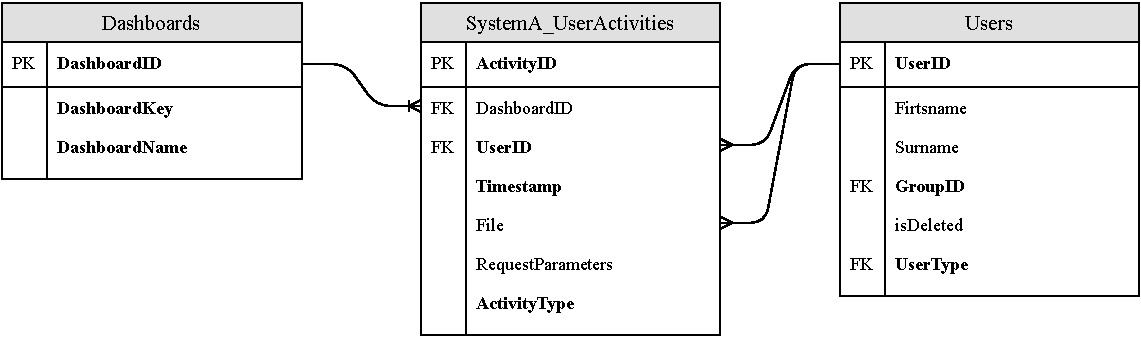
\includegraphics[width=0.9\textwidth]{Images/Chapter2/SystemA_ERD_Basic/SystemA_ERD_Basic.pdf}
	\caption[System A user activity ERD]
	{\textit{System A user activity ERD}}\label{fig:Ch2_SystemA_Basic_ERD}
\end{figure}

\clearpage

In \Cref{fig:CH2_SystemBMetaData} is the meta data JSON for the RequestParameters column in \Cref{tbl:Ch2_System_A_Logging_Points}. This JSON contains certain data parameters important to the event that the user has initiated. This request parameters will need to be specified for each toolbox and dashboard the user events are logged of for System A.

\begin{figure}[!htb]
	\centering
	\begin{lstlisting}[style=JSON] 
	{
		"Parameter1": 4,
		"Parameter2": "Hello World!",
		"Parameter3": true
		"Parameter4": 40.404
	}
	\end{lstlisting}
	\caption[System A meta data JSON]
	{\textit{System A meta data JSON}}\label{fig:CH2_SystemAMetaData}
\end{figure}

\subsubsection{System A logging mechanism design}
\Cref{sec:SystemA_LoggingPoints} the logging points System A's key logging points need to be captured by a logging mechanism. In \Cref{fig:ch2_SystemA_Arch_Design} is the design for the System A's logging mechanism to effectively log the user generated event from the PHP software components. The logging mechanism consist of two main functional requirements (\textbf{F/R}) which is the client and server functional requirements.

\begin{figure}[!htb] % An h :here, t: top, b: bottom.
	\centering % cent the figure
	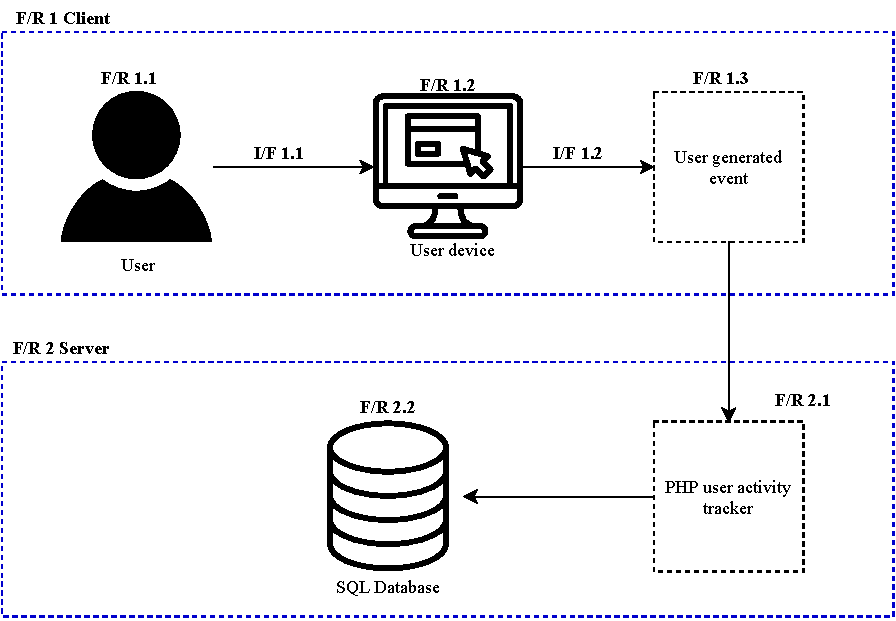
\includegraphics[width=0.9\textwidth]{Images/Chapter2/SystemA_Architecture_Diagram/SystemA_Architecture_Diagram.pdf}
	\caption[System A logging mechanism architecture design]
	{\textit{System A logging mechanism architecture design}}\label{fig:ch2_SystemA_Arch_Design}
\end{figure}

In the client's functional requirements (F/R 1) the user the is main focus and is the initiator of user activity event logs that take place in System A. The user has a direct interface (I/F 1.1) to the device (F/R 1.2) that is currently browsing System A's websites for specific tasks.\par If the user initiates an activity the request will in most cases either be handled in the dashboard manager of System A or on a defined file where the dashboards software components are. These activities are either captured by the logging mechanisms of \Cref{fig:ch2_Dash_PHP_Flow} or \Cref{fig:ch2_DetailView_Flow} that gets the necessary parameters and defines the type of the user generated event of \Cref{tbl:Ch2_SystemA_EventTypes}. \par The user generated event (F/R 1.3) 

\subsubsection{Dash user activty type classification}

In \Cref{fig:ch2_Dash_PHP_Flow} is the process of getting the Dash and Report user activity event type for System A. In System A there are certain software components in a dashboard manager file that manages the dashboards according to which the user has selected to view. This dashboard manager file will always be execute the needed processes to manage the dashboard upon is start-up phase.\par When the user sends a request a to view a dashboard the requested dashboard's ID send to the dashboard manager. The dashboard manager will attempt to get the dashboard based on the provided dashboard ID. If the request doesn't contain a dashboard ID parameter, any attempt to log the activity will be ended and will be handled with the logging process described in \Cref{fig:ch2_DetailView_Flow}. \par If the dashboard ID parameter does exist and is not an empty or null value it will be added to the activity parameters. The activity parameters consist of some of the parameters needed for \Cref{tbl:Ch2_System_A_Logging_Points} when the event log is eventually saved in the database. \par In System A there are reports generated and some of the events of the report generation will use the dashboard manager's file. These user generated events can only be traced there and will send an action parameter that is use to initiate the report generation process.\par The action parameters in System A is parameters set in the Post and Get methods. If the action parameter contains report generation value the activity type needs to be set to the Report user activity type otherwise it is set the Dash user activity type. After the additional parameters and activity type parameters are set the ActivityTracker function is called to complete the log and save it in the SQL database as in \Cref{fig:CH2_SystemA_DB_Iteraction_FlowDiagram}. 

\begin{figure}[!htb] % An h :here, t: top, b: bottom.
	\centering % cent the figure
	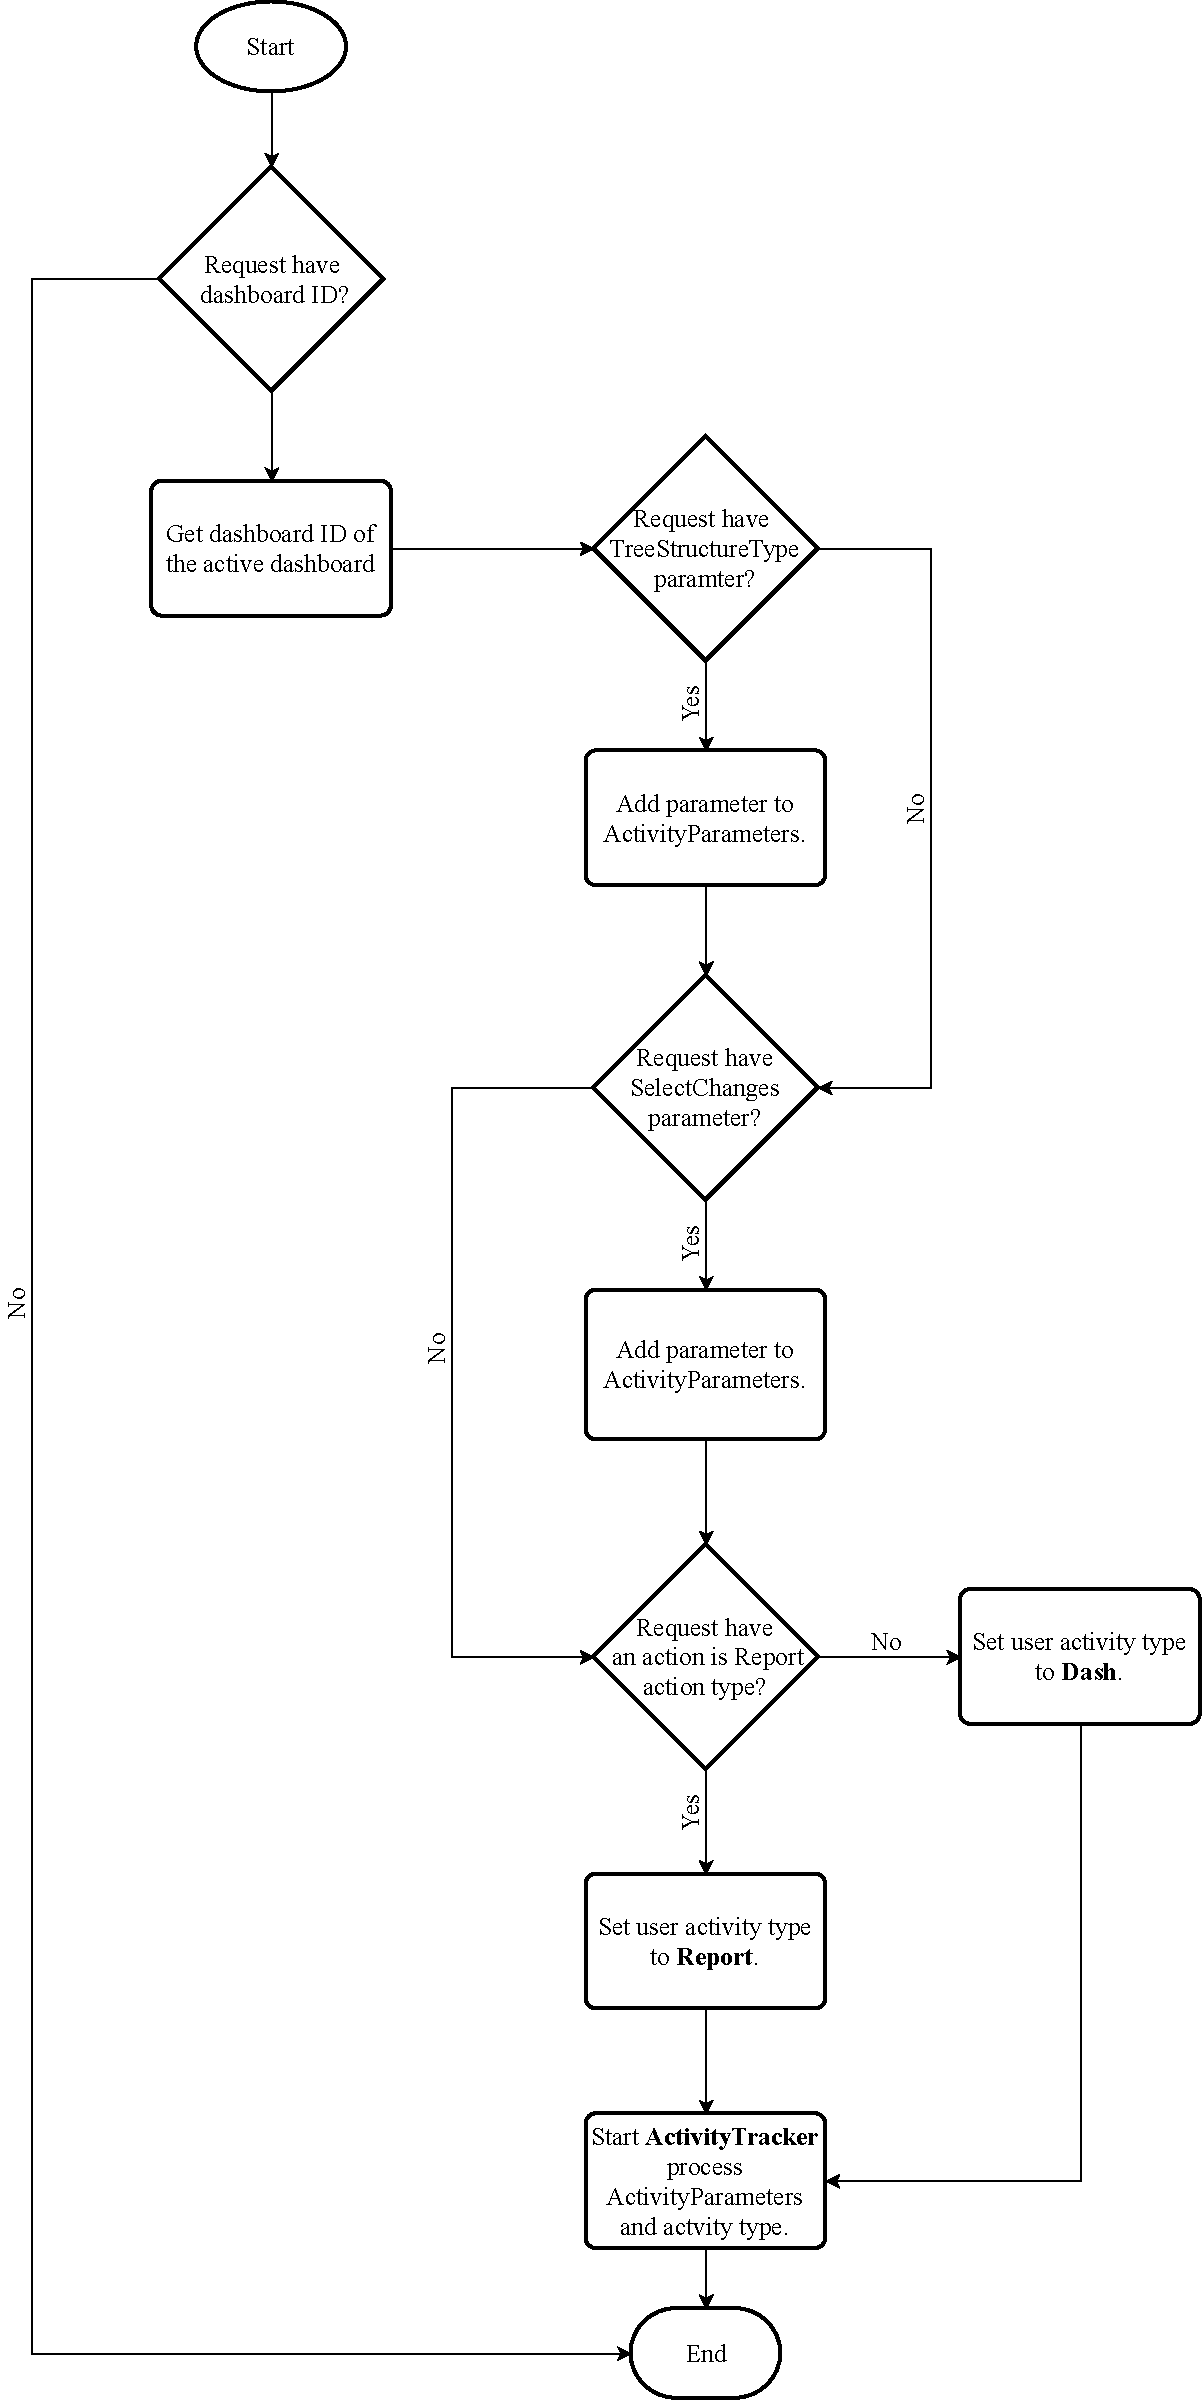
\includegraphics[width=0.7\textwidth]{Images/Chapter2/Dash_PHP_Flow/Dash_PHP_Flow.pdf}
	\caption[User activity logging process in the Dash.php file flow diagram]
	{\textit{User activity logging process in the Dash.php file flow diagram}}\label{fig:ch2_Dash_PHP_Flow}
\end{figure}

\clearpage

\subsubsection{User activity logging process of DetailView and Report event types}

In \Cref{fig:ch2_DetailView_Flow} is the process of getting the DetailView and Report user activity event type for System A. This logging process is used in each file that dashboards are created from. In \Cref{fig:ch2_SystemA_Dashboard} multiple dashboards can use the same files with different configuration parameters send with the request, therefore this significantly reduces the needed development to enable the user activity tracking for the dashboards.\par After the user has navigated to their selected dashboard, any user generated request is logged as user activities in System A. These events can be divided into the DetailView and Report event types based on their action parameters that is send with the request. If the event doesn't have any action parameters, the logging process terminates as this event doesn't count as a valid user activity event.\par If the event does have any action parameters it is checked whether the parameters have report generation value or not. If the event have report action values then the user activity type is set to the Report event type otherwise it is set to DetailView event type.\par There may exist any additional parameters that is send with the request that can be logged. These parameters will vary more than the additional parameters of the Dash events as the Dash events parameters is used to configure the dashboard and not get certain variations activities the user performs on the dashboard.\par If the additional parameters are not null or empty values they are added to the ActivityParameters. With the set ActivityParameters and the defined user activity type the ActivityTracker process of \Cref{fig:CH2_SystemA_DB_Iteraction_FlowDiagram} to create a log entry that is saved in the SQL database.

\begin{figure}[!htb] % An h :here, t: top, b: bottom.
	\centering % cent the figure
	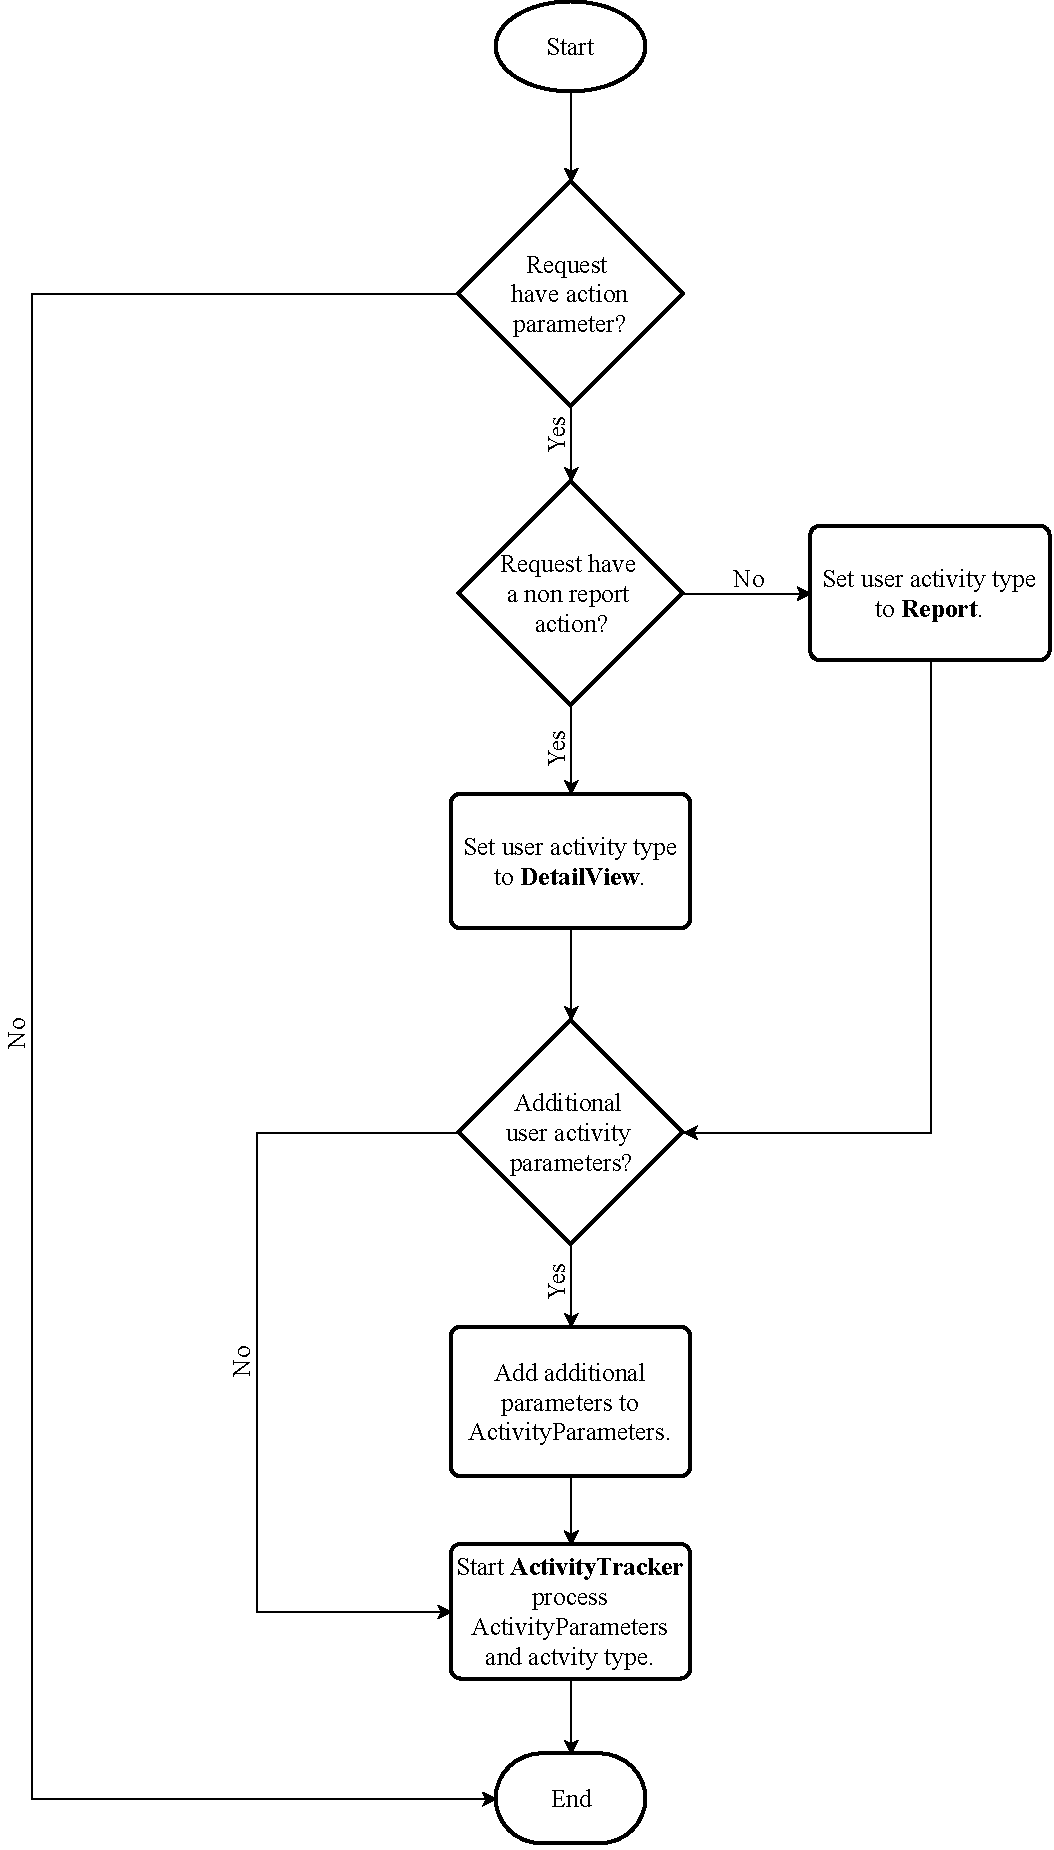
\includegraphics[width=0.75\textwidth]{Images/Chapter2/DetailView_Flow/DetailView_Flow.pdf}
	\caption[User activity logging process of DetailView and Report event types flow diagram]
	{\textit{User activity logging process of DetailView and Report event types flow diagram}}\label{fig:ch2_DetailView_Flow}
\end{figure}

\clearpage

\subsubsection{Database interaction of the logging mechanism}\label{sec:CH2_SystemA_DB_Iteraction_FlowDiagram}

\begin{figure}[!htb] % An h :here, t: top, b: bottom.
	\centering % cent the figure
	\includegraphics[width=0.5\textwidth]{Images/Chapter2/SystemA_ActivityTracker/SystemA_ActivityTracker.pdf}
	\caption[User activity logging process of DetailView and Report event types flow diagram]
	{\textit{User activity logging process of DetailView and Report event types flow diagram}}\label{fig:CH2_SystemA_DB_Iteraction_FlowDiagram}
\end{figure}

\clearpage

\subsection{System B}

\subsubsection{System B's logging points}

In \Cref{fig:ch2_Flow_MVC_Architecture} is a diagram of the request flow of a MVC architecture that shows how the user interacts with it. The user will send multiple request from their own device (client device) via an Internet connection to the server that process the request. The software system will read and write data the database source to create a result that send back to the client device for the user. System B is based on this type of architecture to display multiple menus to the user. 

\begin{figure}[!htb] % An h :here, t: top, b: bottom.
	\centering % cent the figure
	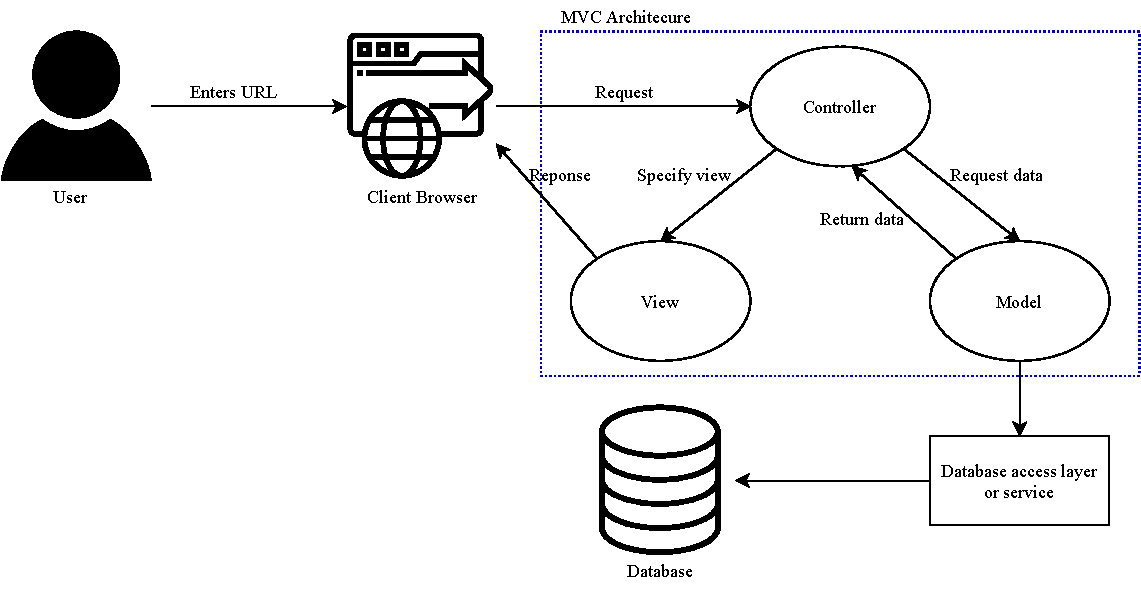
\includegraphics[width=0.95\textwidth]{Images/Chapter2/Flow_MVC_Architecture/Flow_MVC_Architecture.pdf}
	\caption[Request flow in MVC architecture]
	{\textit{Request flow in MVC architecture \cite{Gu2010}}}\label{fig:ch2_Flow_MVC_Architecture}
\end{figure}

In \Cref{sec:SystemA_LoggingPoints} System A mostly relies on the user sessions data to obtain the user generated event's data, for System B this data can be obtained by the FilterContext class in ASP.NET MVC. The FilterContext provides contains the following information about the request:

\begin{itemize}
	\item \textbf{Absolute URI path:} The string containing the absolute URI path the current controller that is active is part of the FilterContext. This does not reference the controller that handles the request but the controller that user is active on before initiating the request. 
	\item \textbf{Absolute request URL:} The request URL contains the controller's name and function that process requests. This reference the controller that handles the request but the controller that user is active on before initiating the request. Most of System B's menus are partitioned in separate units which is called Areas in the ASP.NET MVC projects. The area from which the controller is from is also part of the of this path.
	\item \textbf{Action parameters:} The FilterContext contains action parameters which are the request parameters send with the AJAX request from the client device. These parameters are used in the function that is being called to do certain task within the controller.
\end{itemize}

In System B's session information the user's identification credentials are stored and is used to identify which user initiated the event that is processed.

\clearpage

Using the information from the FilterContext and session of System B the key logging points can be obtained to create \Cref{tbl:CH2_SystemB_LoggingTable} that is saved in SQL database. Each of this logging points can be accessed through a filter action to capture run-time data such as the action parameters that is part of the meta data.

\begin{table}[!htb]
	\centering
	\small
	\caption[System B user activities table]
	{\textit{System B user activities table}}
	\label{tbl:CH2_SystemB_LoggingTable}
	\begin{tabularx}{\textwidth}{|l|l|X|}
		\hline \textbf{Column Name} & \textbf{SQL Data Type} & \textbf{Description} \\
		\hline \textbf{ActivityID} & INT(11) & The activity identification is an incremental number of the event that is logged.\\
		\hline \textbf{Timestamp} & DATETIME & This is the time which the event took place.\\
		\hline \textbf{ActivityType} & ENUM & Each event that the user initiate has an activity type as in \Cref{tbl:Ch2_SystemB_ActivityTypes}. This activity type is dependent if the controller's called method is the index action or based on the HTML element that is part of the meta data. \\
		\hline \textbf{UserID} & INT(4) & Each user has a unique identifier which is a numerical identification number that is foreign key reference to the User table. \\
		\hline \textbf{Area} & VARCHAR(45) & This information is logged to track user activities per Area that represents different software systems that the user can use. \\
		\hline \textbf{Controller} & TEXT & Each event will point back to an controller that process the request. \\
		\hline \textbf{GroupID} & INT(4) & This foreign key reference to the Group table is contract groups identification number. \\
		\hline \textbf{MetaData} & JSON & The meta data of the event contains request parameters, the HTML element from which the request is initiated and other relevant request data of the event. This can also be other meta data is important to get that adds more information about the user's activity using certain controls on System B as in \Cref{fig:CH2_SystemBMetaData}. \\
		\hline
	\end{tabularx}
\end{table}

In \Cref{fig:CH2_SystemBMetaData} the meta data JSON for the user activity log obtained. This JSON contains the request origin of the event from the absolute URI path, HTML element that user used to initiate the event and the request parameters send with the AJAX request. Some of these JSON parameters can be empty depending on the type of the activity.

\begin{figure}[!htb]
	\centering
	\begin{lstlisting}[style=json] 
	{
		"RequestOrigin" : "/Area4/Controller4",
		"RequestElementID" : "Button4",
		"RequestParameters": {
			"Parameter1": 4,
			"Parameter2": "Hello World!",
			"Parameter3": true
			"Parameter4": 40.404
		}
	}
	\end{lstlisting}
	\caption[System B meta data JSON]
	{\textit{System B meta data JSON}}\label{fig:CH2_SystemBMetaData}
\end{figure}

\clearpage

The user activity types in \Cref{tbl:Ch2_SystemB_ActivityTypes} is all of the possible activities the user can generate in System B. The MenuAccessed activity type can be used to track how the user is navigating through the System B just like System A's Dash user activity type. The CustomControls and ElementClickEvents user activity types is the best representation of the system utilisation of System B by the users.

\begin{table}[!htb]
	\centering
	\small
	\caption[System B user activity types]
	{System B user activity types}
	\label{tbl:Ch2_SystemB_ActivityTypes}
	\begin{tabularx}{\textwidth}{|l|X|}
		\hline \textbf{Activity Type} & \textbf{Description} \\
		\hline \textbf{MenuAccessed} & These events are any user activities where the user attempts to access a menu on System B which calls the index method of the menu's controller. In most cases the event request from the client side will be handled by the controller's index function to send back a response of the initial accessing of a specific menu. \\
		\hline \textbf{LogoutAttempt} & Any logout attempt from the user except closing the browser tab or browser. Closing the browser or tab doesn't send any request from the client device back to the server to log that user ended their session. \\
		\hline \textbf{LoginAttempt} & Any user activities on the login page of System B where the user will try enter their credentials to gain access to their user accounts on System B.\\
		\hline \textbf{SessionTracking} & This is any user activities that directly involves extension session due that System B will attempt to logout the user after a hour of inactivity prompting the user to extend their own session.\\
		\hline \textbf{ResetPassword} & Any user activities when the user attempts to reset their password. \\
		\hline \textbf{CustomControls} & System B uses custom controls made the development team, when the user uses these controls it will also initiated an event that can be tracked. \\ 
		\hline \textbf{ElementClickEvents} & Any distinguishable \emph{HTML} element that is clicked by the user that communicates back to the server. These events are ButtonClicked, SelectClicked, ImageClicked, InputClicked, SpanClicked, LabelClicked, ListClicked, HyperLinkClicked, DivClicked, FormInput and GridItem.\\
		\hline
	\end{tabularx}
\end{table}

In \Cref{fig:ch2_SystemB_Basic_ERD} is the ERD of tables directly used for System B. The key logging points of \Cref{tbl:CH2_SystemB_LoggingTable} is used to create the table SystemB\_UserActivities. The data is stored in a SQL database where the Users and Groups tables are. The Users table contains all the information of the users using the System B and the Groups table contains all the mine contract group information. 

\begin{figure}[!htb] % An h :here, t: top, b: bottom.
	\centering % cent the figure
	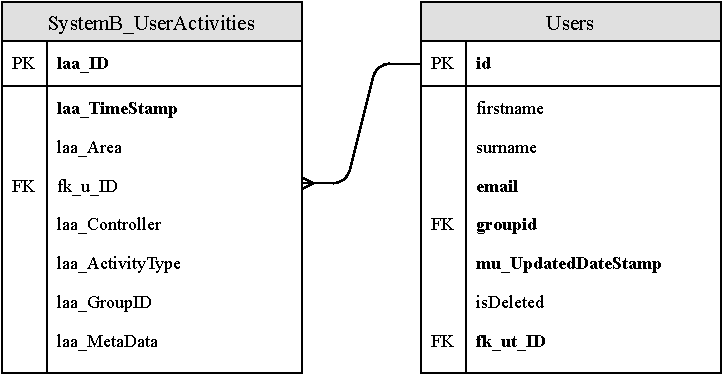
\includegraphics[width=0.99\textwidth]{Images/Chapter2/SystemB_ERD_Basic/SystemB_ERD_Basic.pdf}
	\caption[System B user activity ERD]
	{\textit{System B user activity ERD}}\label{fig:ch2_SystemB_Basic_ERD}
\end{figure}

\clearpage

\section{System utilisation analysis}

\section{Integration}
In this section the integration of the utilisation analysis and logging mechanism will be discussed.

\section{Conclusion}
Conclude the chapter about the development of the logging mechanism and utilisation analysis.
\chapter{Results}
\label{chap:3}
\ChapterPageStuff{3}

\section{Introduction}
In \Cref{sec:ch2_preamble}, the methodology was created for a web-based software system. As described in this section, a user can have multiple systems and subsystems linked to their account. The implementation is done for multiple software systems in this section. The system implementation will focus more on the development of the logging mechanism, and the critical analysis will prioritise software maintenance using a utilisation analysis.

\section{Implementation and verification}
To implement the development of solution that is discussed in \Cref{sec:ch2_developementOfSolution} will be implemented and verfied on a test system. The test system is created in a \texttt{APS.NET Core Web SDK} software environment. 

\subsection{System Implementation}

\subsubsection{Log attibutes}\label{sec:ch3_logAtrributes}
Using the functional requirements discussed in \Cref{sec:ch2_logAttributesRequirements} data columns is made for the user based event's log attributes. These log attributes for a structured database is defined in \Cref{tbl:ch3_Log_Attributes}. 

\begin{table}[!htb]
	\centering
	\caption[Logging attributes]
	{\textit{Logging attributes}}
	\label{tbl:ch3_Log_Attributes}
	\begin{tabularx}{\textwidth}{|l|l|X|}
		\hline \textbf{Column name} & \textbf{Requirement ID} & \textbf{Description}\\
		\hline \texttt{laa\_ID} & \ref{fr:lpa1} & User based actvity identifier. \\
		\hline \texttt{laa\_TimeStamp} & \ref{fr:lpa2} & Timesstamp when the activity has occur. \\
		\hline \texttt{laa\_ActivityType} & \ref{fr:lpa3} & Activity type of the log event. \\
		\hline \texttt{fk\_u\_ID} & \ref{fr:lpa4} & Identification number of the user associated with the log event. \\
		\hline \texttt{laa\_Area} & \ref{fr:lpa5} & System where the activity has occur. \\
		\hline \texttt{laa\_Controller} & \ref{fr:lpa5} & Subsystem where the activity has occur. \\
		\hline \texttt{laa\_MetaData} & \ref{fr:lpa6} & Metadata captured from the \textit{HTTP request}. \\
		\hline \texttt{fk\_g\_ID} & \ref{fr:lpa7} & Additional identifiers for the log event. \\
		\hline
	\end{tabularx}
\end{table}



\begin{lstlisting}[style=json, caption={\textit{Metadata JSON}}, label={fig:ch3_MetadataJson}] 
	{
		"RequestOrigin": "/System/Subsystem1/",
		"RequestElementID": "ButtonSaveCsv",
		"RequestParameters": {
			"aTagIDs": [
				"6284",
				"20320"
			],
			"aToDate": "2020-04-06",
			"aGroupID": 2,
			"aFromDate": "2020-03-30"
		}
	}
\end{lstlisting}

\begin{landscape}
	\begin{figure}[!htb] % An h :here, t: top, b: bottom.
		\centering % cent the figure
		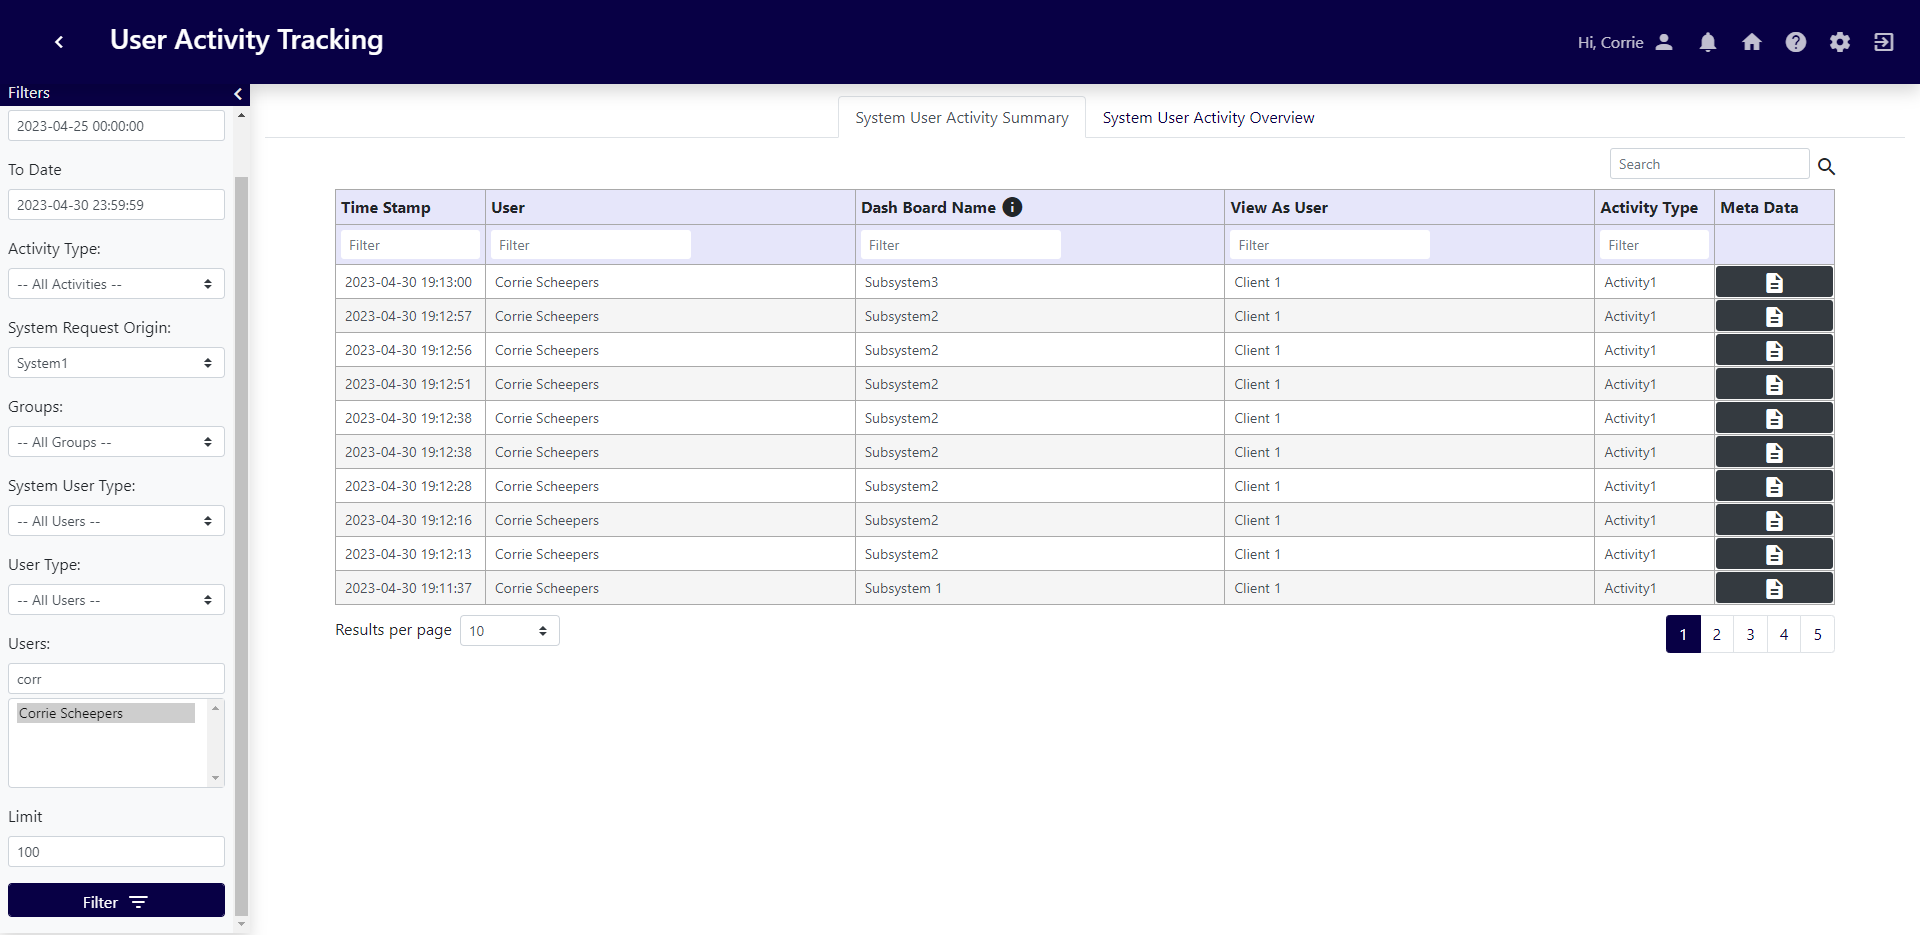
\includegraphics[width=0.99\linewidth]{img/ch3/analysis/UAT_menu.png}
		\caption[Interactive user actvity viewer]
		{\textit{Interactive user actvity viewer}}\label{fig:ch3_UAT_menu}
	\end{figure}
\end{landscape}

\subsubsection{Obtaining the element of user-based event}\label{sec:ch2_ElementObtaining}
In \Cref{sec:ch2_webApplicationArchitecture} the user-based activity event will be use a \textit{HTTP request} to send to the server when the user interacted with an \textit{HTML element}. For the functional requirements activity type (F/R 1.5.3) and metadata (F/R 1.5.6) in \Cref{tbl:ch2_keyLoggingAttributes} the \textit{HTML element} needs to be obtained to get the element's tag and identification text. This can be difficult to obtain due to \textit{bubbling}\footnote{\textbf{Bubbling} is when an event happens on an element, it first runs the handlers on it, then on its parent, then up on other ancestors. \cite{EventBubbling}.} that may occur when searching for the element that the user specifically interacted with.\par In \Cref{fig:ch2_event_bubbling} is the event propagation example of a child element that has been clicked on which executes a DOM event. The event propagation consists of three phases~\cite{EventBubbling}:

\begin{itemize}
	\item \textit{Capturing phase:} The event propagates downwards to the targeted element that the user interacted with.
	\item \textit{Target phase:} The event reaches the targeted element to execute the DOM event.
	\item \textit{Bubbling phase:} The event bubbles up from the targeted element
\end{itemize}

\begin{figure}[!htb] % An h :here, t: top, b: bottom.
	\centering % cent the figure
	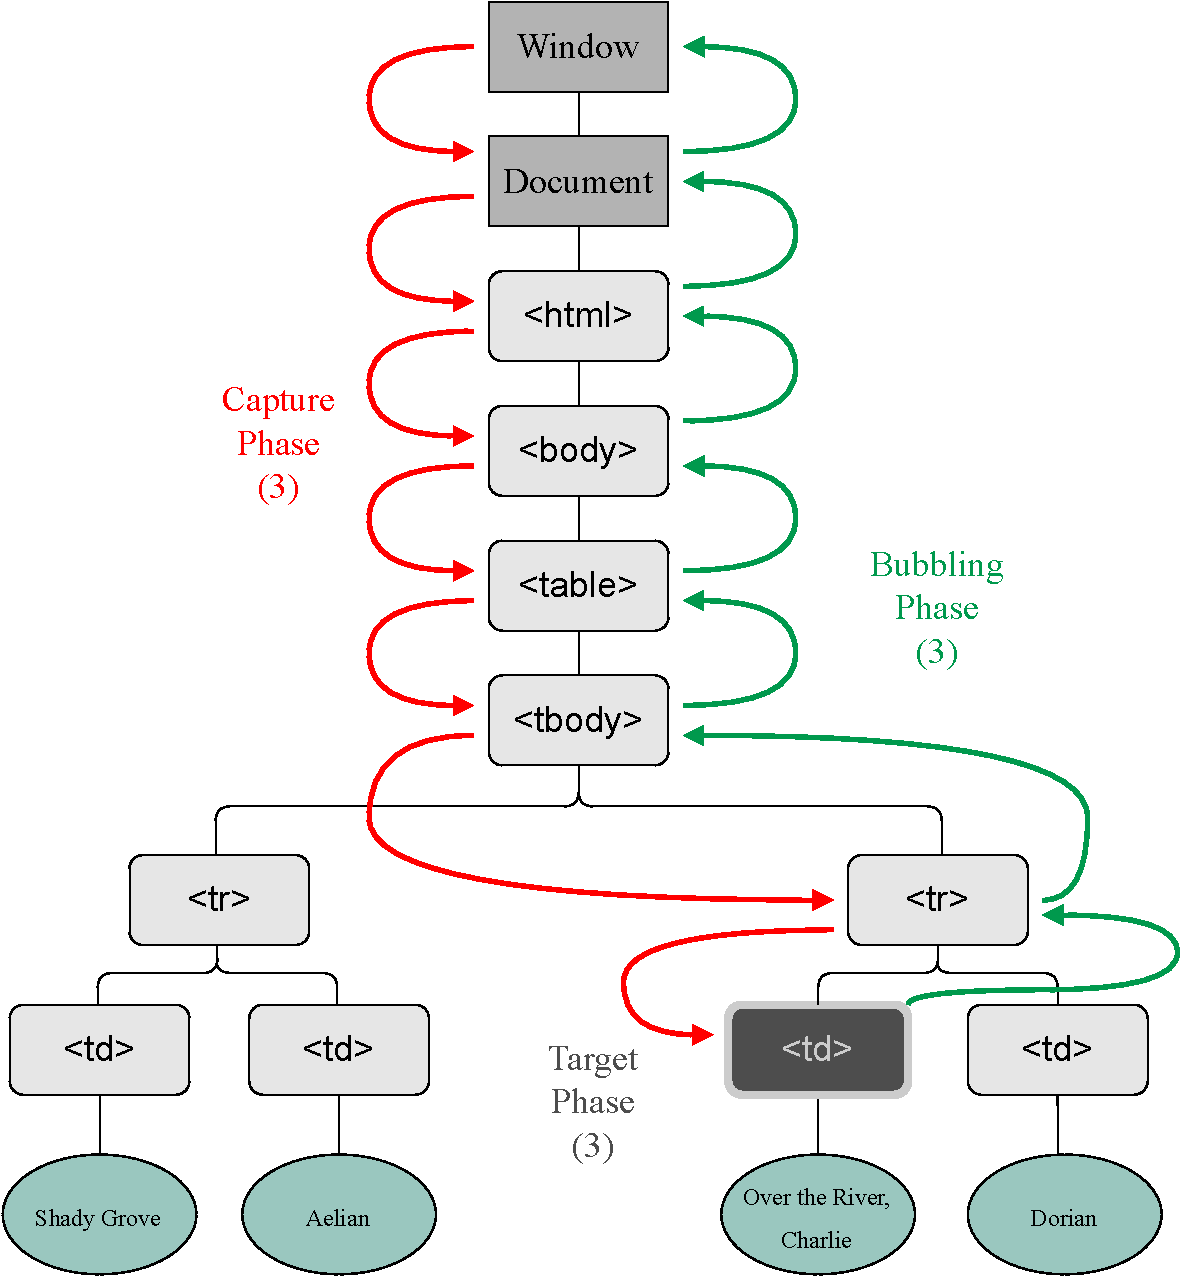
\includegraphics[width=0.6\textwidth]{Chapter2/event_bubbling/event_bubbling.pdf}
	\caption[JavaScript event propagation]
	{\textit{JavaScript event propagation~\cite{EventBubbling}}}\label{fig:ch2_event_bubbling}
\end{figure}

Capturing the targeted element may be difficult as some Web pages may have more complex HTML where the event propagation may sometimes not obtain the correct element information which the user interacted with. Another DOM event may have started during the initial element's event, therefore it is more accurate to obtain the targeted element by obtaining the last known element the user hovered over on the user interface.\par In \Cref{fig:ch2_element_event_capturing} is the flow diagram to capture the element user interacted with for the user-based activity log. This code segment will be initiated during the \texttt{beforeSend} operation of the \textit{AJAX request} to filter HTML elements by predefined allowed elements to use. Filtering the element tag names ensures that unwanted more complex elements or more basic elements that are not expected to be the initiator of the event will be used. \par If the Web location already changed or no element exists, the contents of the page might have already changed during the event propagation. The last known element that the user hovered on must be used as most likely might have been the element that the user interacted with. This will ensure there is always an element that has been detected and parsed with the request header in most UI changes.

\clearpage

\begin{figure}[!htb] % An h :here, t: top, b: bottom.
	\centering % cent the figure
	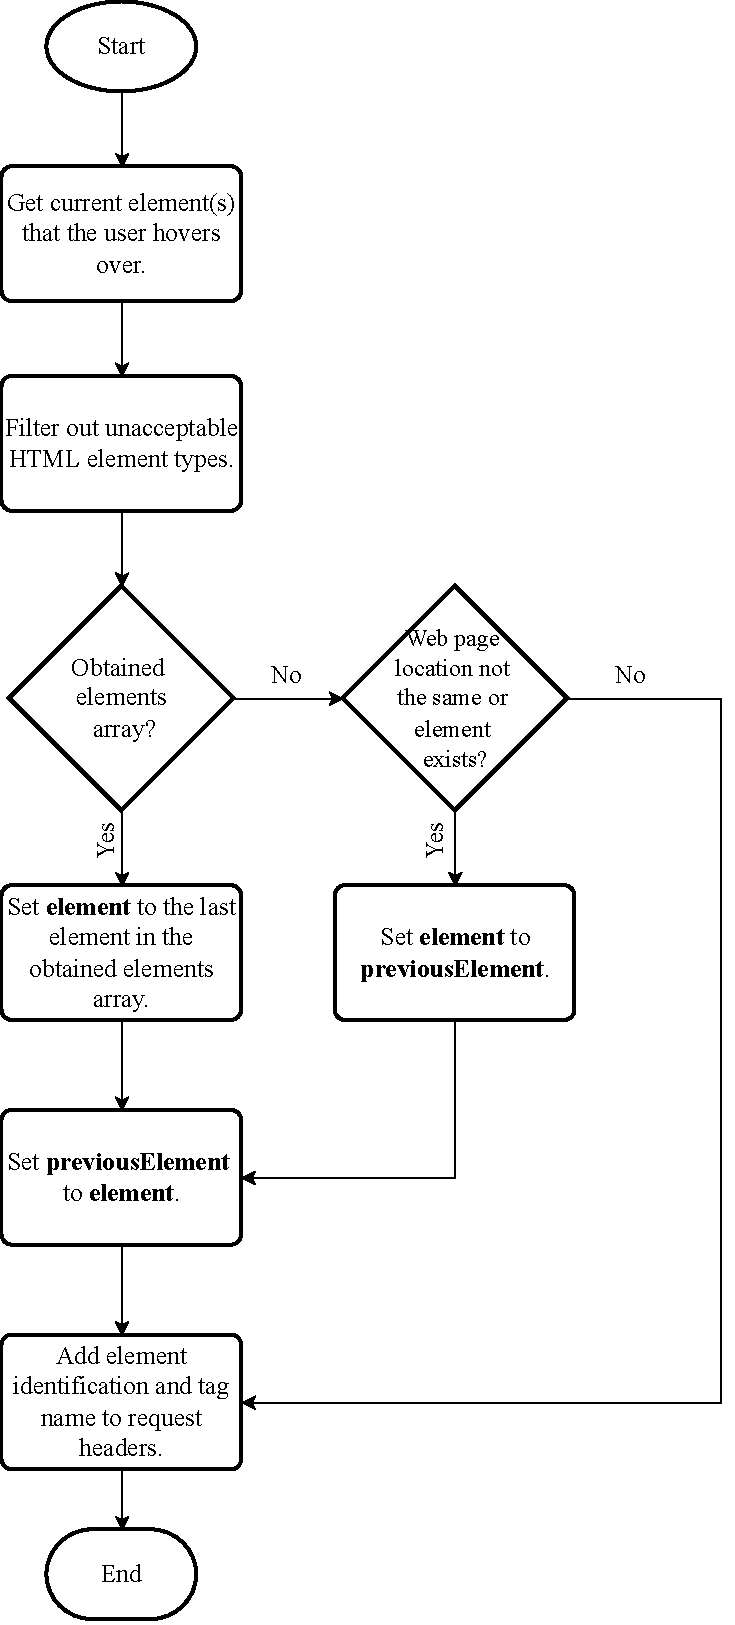
\includegraphics[width=0.5\textwidth]{Chapter2/element_capturing/element_capturing.pdf}
	\caption[HTML element capturing flow diagram]
	{\textit{HTML element capturing flow diagram}}\label{fig:ch2_element_event_capturing}
\end{figure}

\clearpage

\subsubsection{Log attributes}

\section{Case studies}

\subsection{Case study identification}

\subsection{Case study results}

\subsubsection{System A results}

\begin{landscape}
	\begin{figure}[!htb]
		\centering % cent the figure
		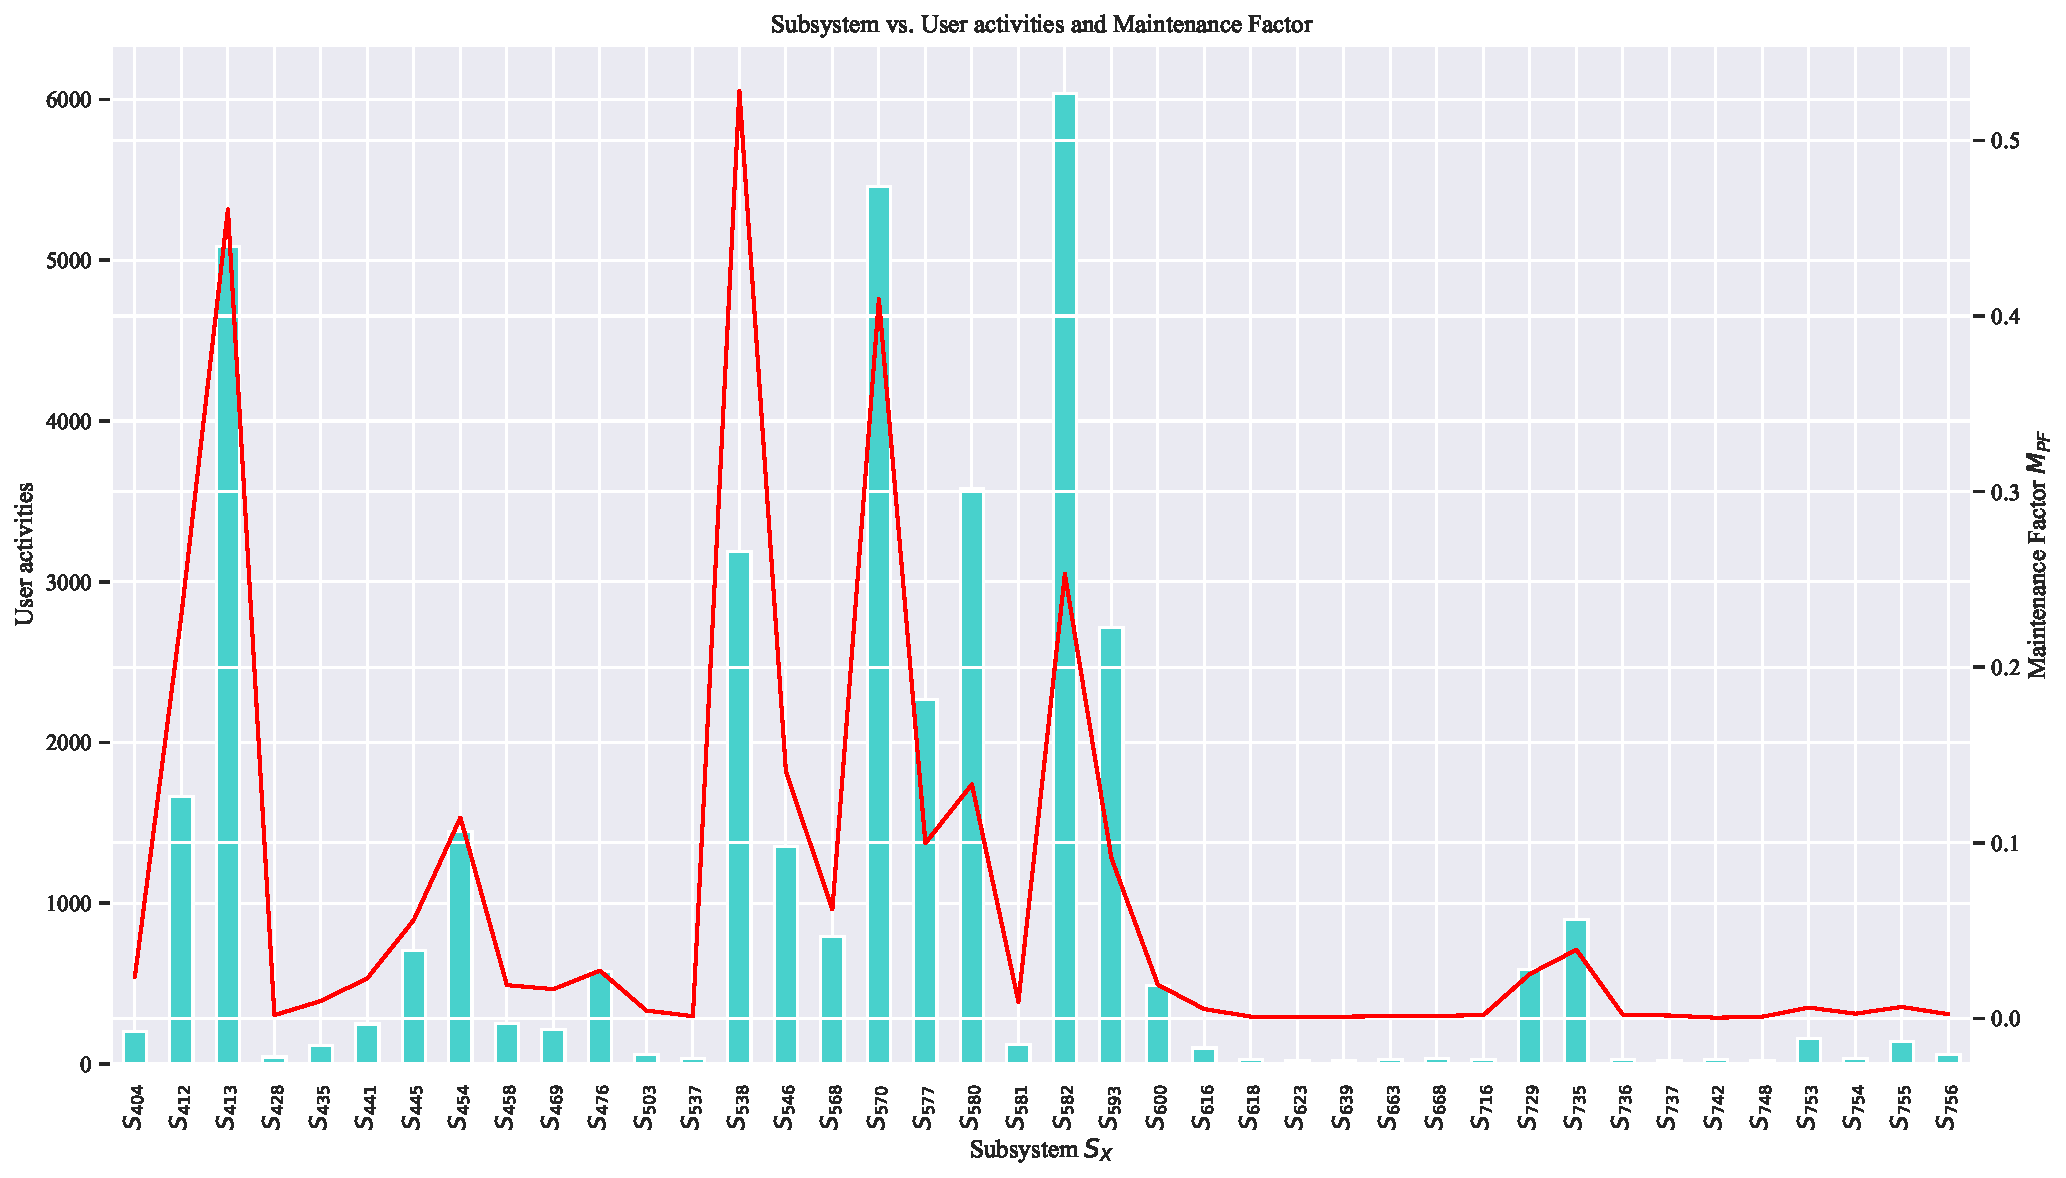
\includegraphics[width=0.95\linewidth]{img/ch3/analysis/case_A_subsystems_1.pdf}
		\caption[Case study 1 subsystem activities part 1]
		{\textit{Case study 1 subsystem activities part 1}}\label{fig:ch3_saS1S246}
	\end{figure} 
\end{landscape}

\subsubsection{System B results}

\begin{landscape}
	\begin{figure}[!htb]
		\centering % cent the figure
		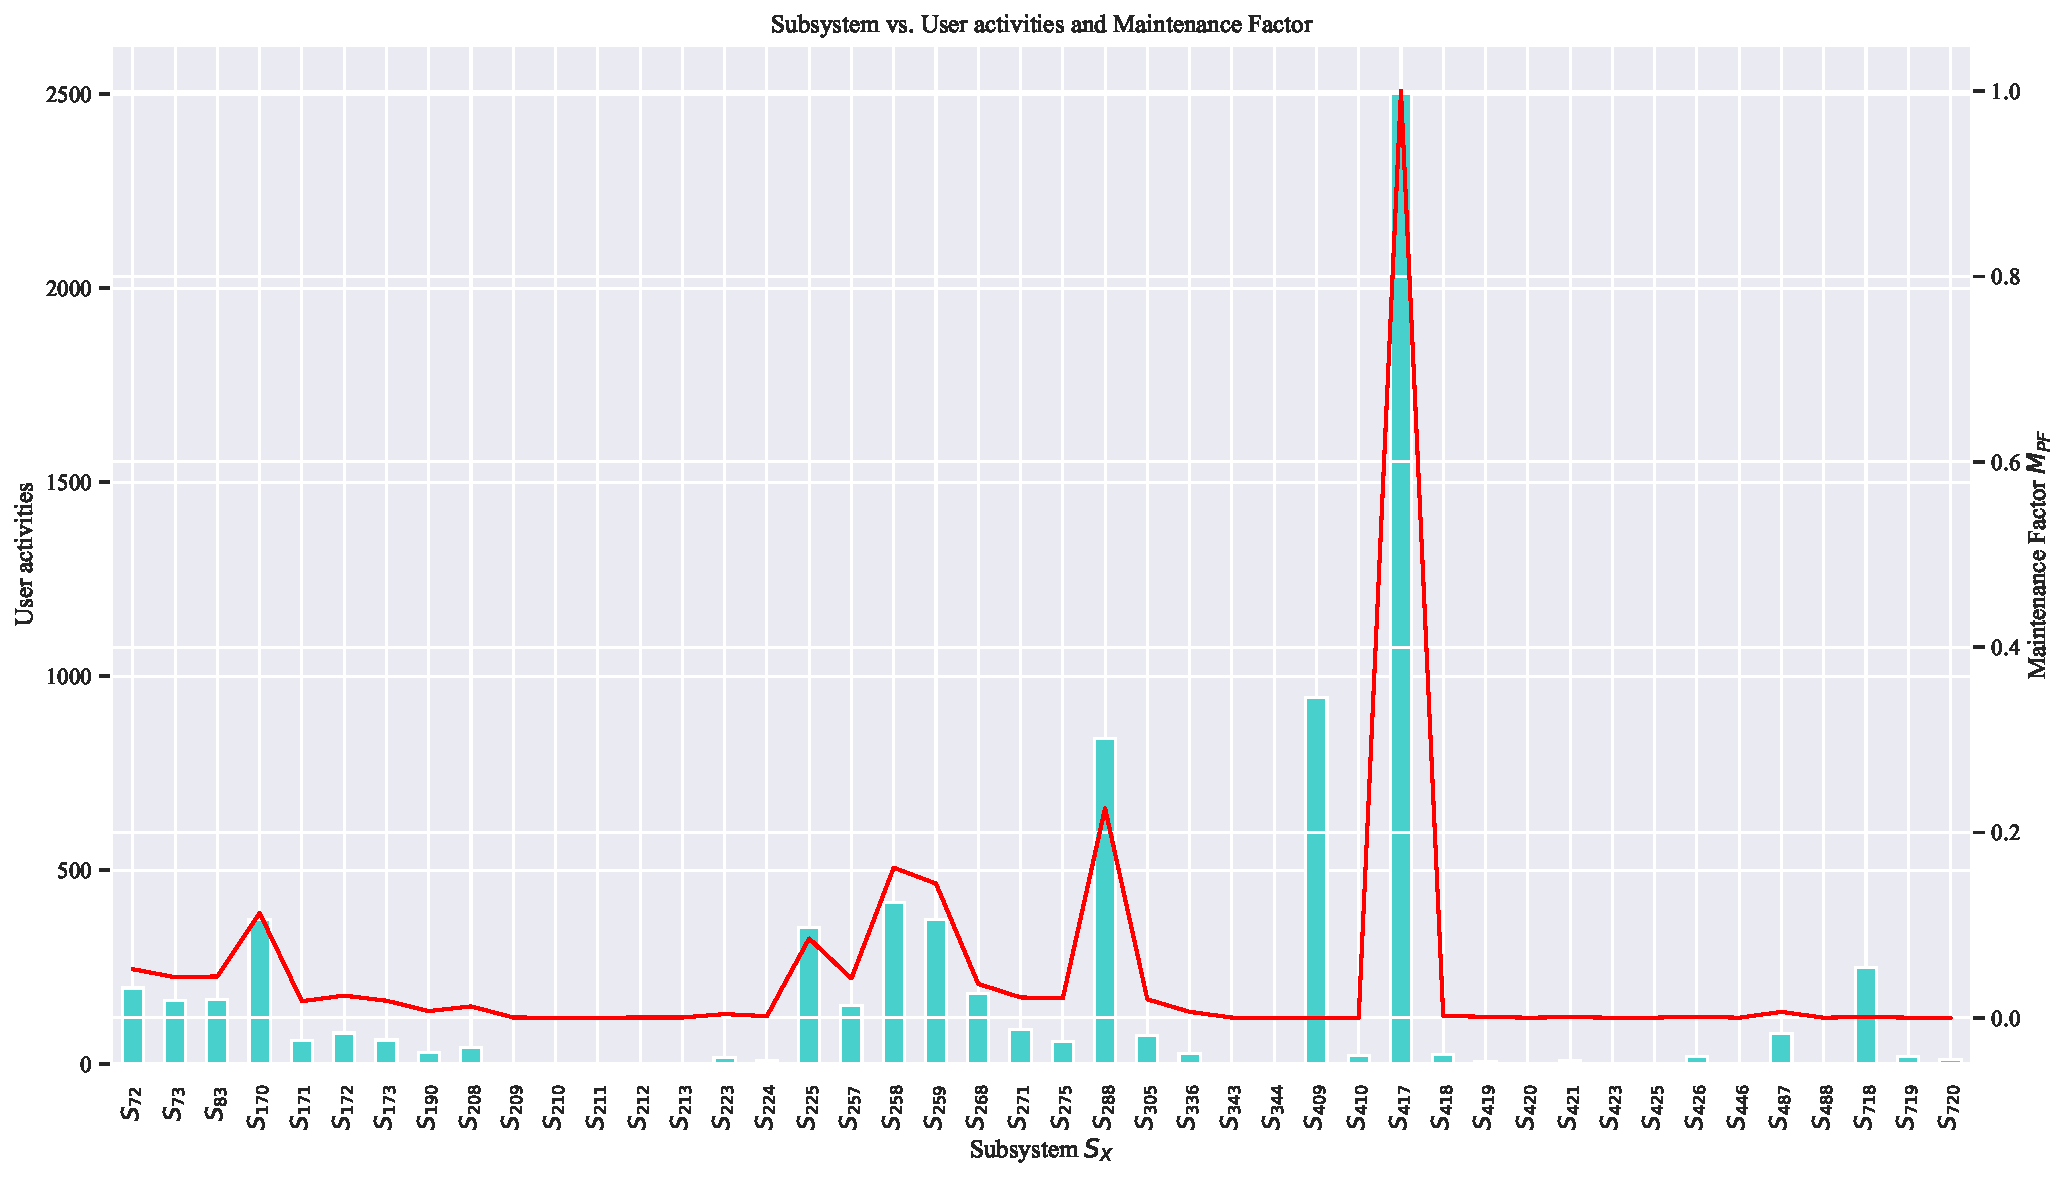
\includegraphics[width=0.95\linewidth]{img/ch3/analysis/case_B_subsystems_1.pdf}
		\caption[Case study 1 subsystem activities part 1]
		{\textit{Case study 1 subsystem activities part 1}}\label{fig:ch3_saS1S24}
	\end{figure} 

	\begin{figure}[!htb]
		\centering % cent the figure
		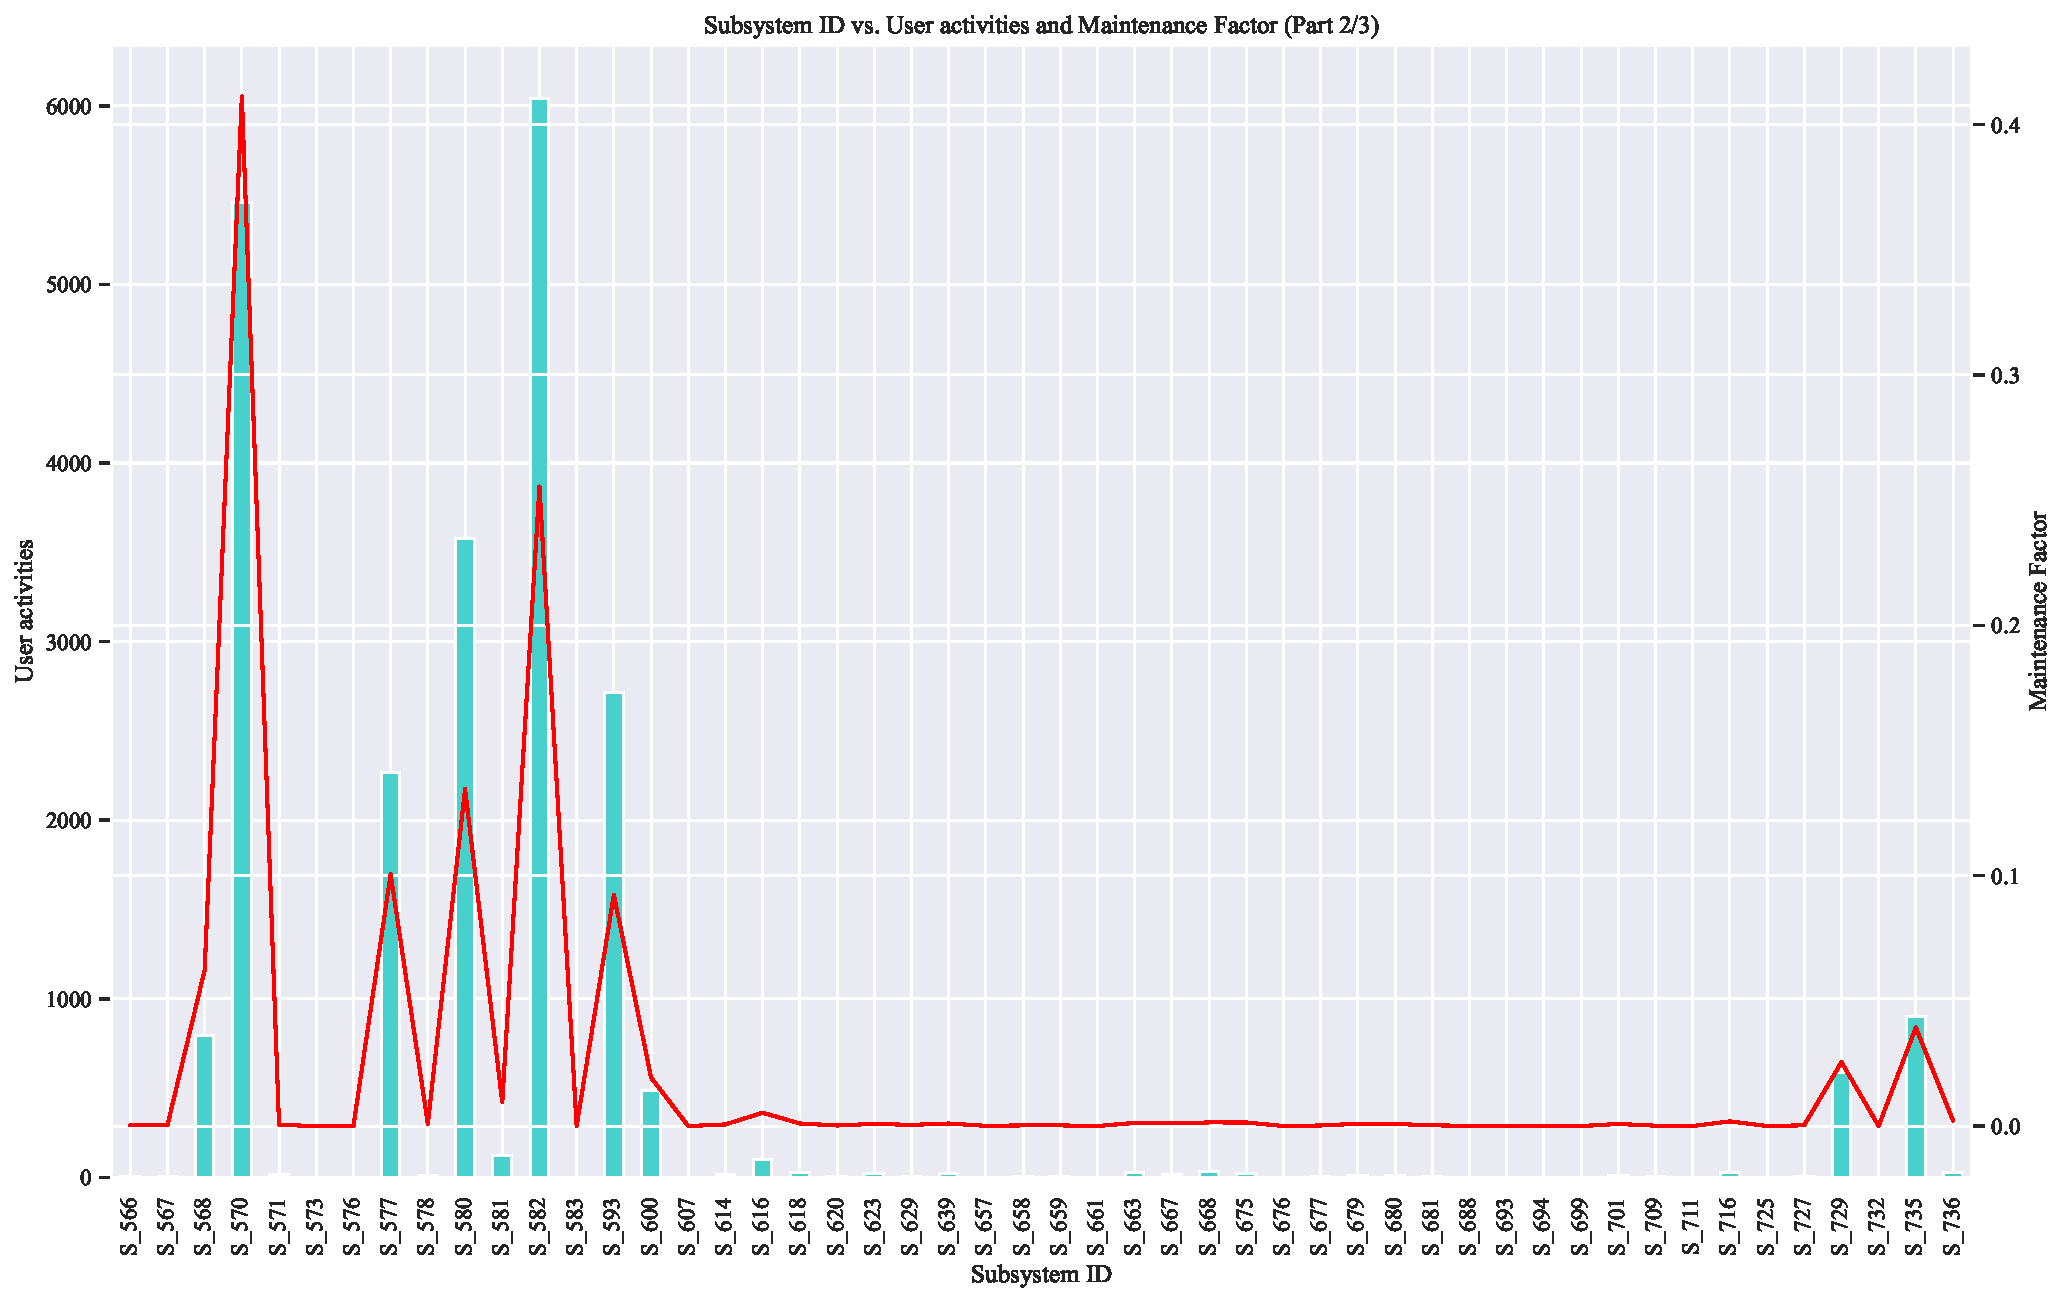
\includegraphics[width=0.95\linewidth]{img/ch3/analysis/case_B_subsystems_2.pdf}
		\caption[Case study 1 subsystem activities part 1]
		{\textit{Case study 1 subsystem activities part 1}}\label{fig:ch3_saS1S25}
	\end{figure} 

	\begin{figure}[!htb]
		\centering % cent the figure
		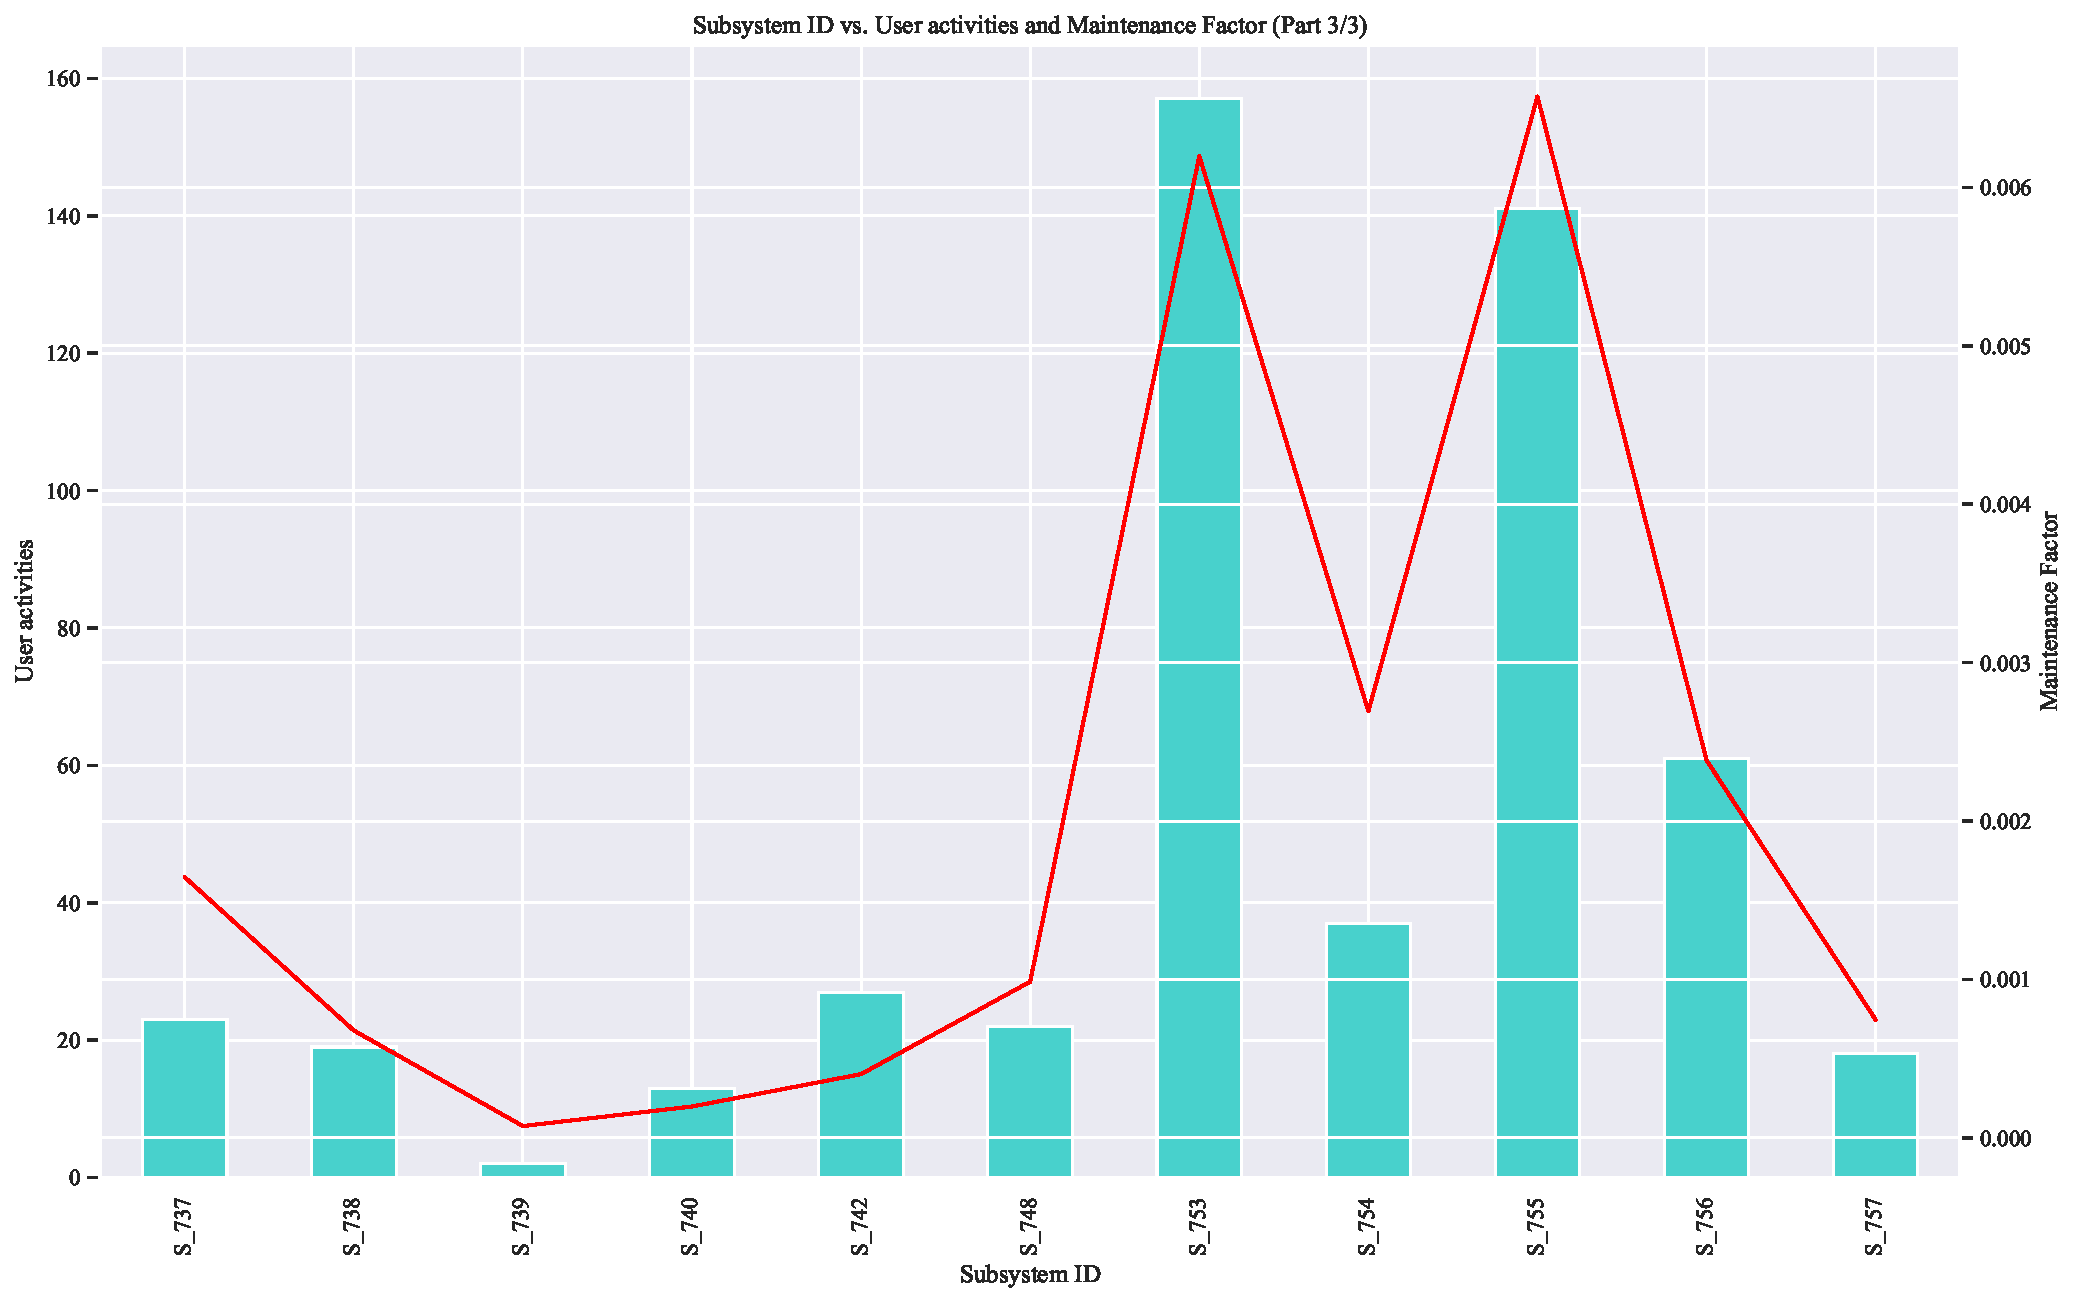
\includegraphics[width=0.95\linewidth]{img/ch3/analysis/case_B_subsystems_3.pdf}
		\caption[Case study 1 subsystem activities part 1]
		{\textit{Case study 1 subsystem activities part 1}}\label{fig:ch3_saS1S26}
	\end{figure} 
\end{landscape}

\clearpage

\subsection{Critical analysis results}

\section{Conclusion}
\chapter{Conclusion}
\label{chap:4}
\ChapterPageStuff{4}

\section{Discussion}

\subsection{Contributions made to literature}
\Cref{chap:1} highlighted the importance of software maintenance in the entire life cycle of most software systems. It is an essential task in the Software Development Life-Cycle that will use up to $60\%-80\%$ of the total available software resources.\par In \Cref{sec:ch1_softwareMaintenanceIntro}, it has been identified that software maintenance should be efficiently implemented due to its high resource cost. Prioritisation of software maintenance can improve the software maintenance efforts of developers more efficiently. Event logging has been identified as a proven method for prioritisation of software maintenance.\par An extensive literature study revealed three State of the Art topics for this study: software maintenance, event logging and log analysis. In \Cref{tbl:ch1_stateOfTheArt2}, the State of the Art further highlighted the gap in the existing literature. Especially in event logging, where it is mainly used for system diagnostics.\par The method in \Cref{chap:2} it has been identified that the event logging should be made explicitly for the log analysis. Additional functional requirements were made for a user-based logging mechanism using existing logging practices defined in the literature. This method contributes to the literature by creating these functional requirements that the logging mechanism needs to be able to meet for software maintenance prioritisation. \par The software maintenance literature mainly focused on the optimisation of the actual software maintenance tasks or the implementation of the software maintenance models. The value added to the literature is the method used in \Cref{chap:3} to make maintenance prioritisation recommendations using a log analysis on the obtained logs. A maintenance priority factor was created in this log analysis to make these recommendations.\par The method was verified by implementing it on a test system in \Cref{sec:ch3_implementation,sec:ch3_Verification}. The verification proved that the method could make software maintenance prioritisation by comparing the input with the expected output.\par After verifying the method, it was implemented in three case studies. These case studies consisted of software systems with other operational use cases and software environments to evaluate the results of the method. The functional requirements defined by the technique were mainly satisfied in each case to study to create the software maintenance prioritisation successfully.\par These results are evaluated, and the method's shortcomings were identified for each case study. Each case was also compared to the other after their in-depth analysis.

\clearpage

\subsection{Value added to industry}
The method in \Cref{chap:2} is used on different case studies in \Cref{sec:ch3_caseStudies}. Each of these case studies explored the various applications of the generic logging mechanism to obtain user-based events. The results proved that the logging mechanism could get the desired user-based activities. However, additional adaptions were needed for each case study to ensure the log quality was acceptable for consistent, reliable log analysis.\par These adaptations were due to the software environment (software languages and design methodologies used) and the purpose of the software system. Older systems had to use different logging points to yield the same result as newer software systems that can use less or one logging point.\par These systems used the same user-based event type with similar operational software use cases. Systems with the same software architecture but different functional use cases also had various adaptations to their logging mechanism. These adaptions ensured that the desired log attributes were correctly obtained for the log analysis. \par The maintenance prioritisation recommendations for each study case used the defined generic methodology. The log analysis for each case study was similar as the log requirements for the user-based utilisation for all the case studies were only different for each of their user-based event types. These user-based event types represent the operational use cases for the case study to further observe the kind of utilisation of the subsystems. \par The results proved that the generic methodology defined in \Cref{chap:2} could be implemented on different software systems with other operational use cases for each case study. In the web development industry, similar software systems as the case study or other software systems will benefit from implementing this methodology to improve software maintenance decisions using these recommendations for prioritisation.

\subsection{Validation strategy}
\Cref{tbl:ch4_ValidationStart} is the validation strategy used for this study. Each of the literature and empirical objectives, respectively, in \Cref{sec:ch1_empiricalObjective,sec:ch1_literatureObjective} is validated in the section it was met.

\clearpage

\begin{table}[!htb]
	\centering
	\caption[Study validation]
	{\textit{Study validation}}
	\label{tbl:ch4_ValidationStart}
	\begin{tabularx}{\textwidth}{Xp{3cm}p{3cm}}
		\toprule
		\textbf{Objective}  & \textbf{Section} & \textbf{Objective met} \\ \midrule
		\textbf{Literature Objectives:} & & \\ \midrule
		\rowcolor{lightgray}
		\RaggedRight \objAi & \RaggedRight \Cref{sec:ch2_logAttributesRequirements,sec:ch2_webApplicationArchitecture} & \cmark \\
		\RaggedRight \objAii & \RaggedRight \Cref{sec:ch2_loggingPoints,sec:ch2_webApplicationArchitecture} & \cmark \\
		\rowcolor{lightgray}
		\RaggedRight \objAiii & \Cref{sec:ch2_logAnalysisTools} & \cmark \\ 
		\RaggedRight \objAiv & \Cref{sec:ch2_utilisationImprovements} & \cmark \\ \midrule
		\textbf{Empirical Objectives:} & & \\ \midrule
		\rowcolor{lightgray}
		\RaggedRight \objBi: 
			\begin{enumerate}
				\item \objBiSubA
				\item \objBiSubB
				\item \objBiSubD
				\item \objBiSubC
			\end{enumerate} & \Cref{sec:ch3_implementation} & \cmark \\
		\RaggedRight \objBii & \Cref{sec:ch3_Verification} & \cmark \\
		\rowcolor{lightgray}
		\RaggedRight \objBiii & \Cref{sec:ch3_caseStudies} & \cmark \\
		\bottomrule
	\end{tabularx}
\end{table}


\section{Recommendations}
In \Cref{sec:ch3_caseStudies}, the case studies highlighted the limitations of the methodology used. The functional requirements can be expanded on the process to improve the method.

\subsection{Logging quality}
\Cref{sec:ch1_loggingQuality} described the event log quality as an essential part of the logging mechanism. The event logs must be accurate, manage complex structures, and be consistent and complete. For the methodology used, not all of the dimensions of \Cref{fig:ch1_EventQModel} are used to design the logging mechanism.\par This presents Case Study B's logging points functional requirement (\ref{fr:loggingPoints}). The multiple logging points introduced inconsistencies in the event logs for the groups of subsystems used. There are studies on improving event log quality, but creating an event log quality model specifically for user-based event logging can increase the log quality. \par Some of the defined event log quality model requirements defined in \Cref{fig:ch1_EventQModel} still need to be fully integrated into the method. Some of these requirements can add value to the logging quality.

\subsection{Maintenance prioritisation}
The maintenance prioritisation (\ref{fr:maintenancePrioritising}) can have improvements made in multiple ways. The \Cref{eq:ch2_maintenanceFactorSimplified,eq:ch2_eventNormalised,eq:ch2_priorityNormalised} makes use of the full user-based event logs per subsystem and total users linked per system as its base variables.\par From the results observed of the case studies in \Cref{sec:ch3_caseStudies}, the base variables had an overwhelming impact on the prioritisation factor. Introducing other variables that represent other factors from the log attributes can improve the accuracy of the maintenance prioritisation. One important variable that could have been used is the user activity type of each case study.

\subsubsection{User activity types}
Throughout the study, the user activity type was essential to describe what can be classified as a user event. This primary log attribute can add another dimension to the results, as some user activities may be more important than others. \par For software systems, as in Case Study C, where most user activity types were grouped, can benefit the final results. There are a few differences between some activity types. 

\subsubsection{User and activity parameters}
\par Normalisation is used in \Cref{eq:ch2_maintenanceFactorSimplified,eq:ch2_eventNormalised,eq:ch2_priorityNormalised} to make a comparable scale for both of the main variables for the software maintenance prioritisation. While Normalisation yielded similar results, there were numerous outliers on each variable's low and high ends. The data does not follow a specific distribution or pattern as $S_{582}$ of Case Study A with a normalised activity of 1. This subsystem had the highest normalised activity but the $4^{th}$ highest maintenance priority due to its lower unique active user base.\par Using different techniques to formulate a software maintenance priority factor may have placed $S_{582}$ higher. If the effect of the total unique users were not used as the primary prioritisation factor for this situation. 

\clearpage

\section{Conclusion}

\subsection{In summary}
\begin{itemize}
	\item There is a need to improve software maintenance activities in the industry, but software maintenance prioritisation is still a problem for most software developers.
	\item Event-based logging is a proven method to get valuable information about a software system.
	\item A log analysis of the utilisation of the software system can provide the needed evidence to prioritise software systems based on the extracted log data.
	\item Creating a user-based event logging mechanism to implement a system utilisation log analysis is a solution to the identified problem.
	\item Three different case studies with two different operational use cases verified the designed methodology for this study.
\end{itemize}

\subsection{In conclusion}
Analysing user-based event logs can enhance software maintenance resource management by prioritising maintenance tasks through a comprehensive log analysis.
%%@@@@@@@@@@@@@@@@@@@@@@@@@@@@@@@@@@@@@@@@@@@@@@@@@@@@@@@@@@@@@@@@@@@@@@@@@@@@@@@@@@@@@@@@@@@@@@@@@@@
%@@        Chapter 5: Discussion                                                                  @@
%@@@@@@@@@@@@@@@@@@@@@@@@@@@@@@@@@@@@@@@@@@@@@@@@@@@@@@@@@@@@@@@@@@@@@@@@@@@@@@@@@@@@@@@@@@@@@@@@@@@

\chapter{Discussion}
\label{chap:5}
\ChapterPageStuff{5}

\section{Preamble}
%TODO More Information in this section. Introduce the rest of the chapter
%TODO Too Specific 
In this chapter, the methodology to create and implement a logging mechanism to do system utilisation analysis on software system will be discussed. \Cref{sec:ch1_eventLogging} provided the necessary literature to create a logging mechanism in \Cref{sec:Ch3_LoggingMechanism} for two software systems.

\section{Logging mechanism}\label{sec:Ch3_LoggingMechanism}
For this study two software systems are used to implement two different logging mechanisms. The first software system which will be called System A, is an energy management system that uses \emph{PHP}. System B is a \emph{.NET Framework}\footnote{\label{ftn:NetFramework}\textbf{.NET Framework} is a run-time execution environment that consists of common language run-time (\emph{CLR}) and a \texttt{.NET Framework Class Library} \cite{Harkness2007}.} system with a \emph{MVC} architecture as in \Cref{fig:ch2_Flow_MVC_Architecture} and is the administrative software system to configure System A.

\clearpage

\subsection{System A}
Logging point is essential data that describes the event's key features when creating a log as discussed in \Cref{sec:ch1_loggignPoints}. Both System A and B have certain key logging points that need to be obtained from the user-generated event.

\subsubsection{System A's logging points}\label{sec:SystemA_LoggingPoints}
In \Cref{fig:ch2_SystemA_Dashboard} each mine group have multiple toolboxes linked to them. They can be the same toolbox linked to both mine groups such as \emph{T1} and \emph{T3}. These toolboxes represent a group of dashboards related to the aspects of energy management of mines.\par Each of these toolboxes have a dashboards linked to them and each mine group can have different dashboards linked to the to the same toolbox. Each one of these mine groups, toolboxes and dashboards forms part of System A's web pages which the user can access where event logs are generated.

\begin{figure}[!htb] % An h :here, t: top, b: bottom.
	\centering % cent the figure
	\includegraphics[width=0.8\textwidth]{Chapter2/SystemA_Dashboard/SystemA_Dashboard.pdf}
	\caption[System A dashboard links]
	{\textit{System A dashboard links}}\label{fig:ch2_SystemA_Dashboard}
\end{figure}

\clearpage

Each dashboard in \Cref{fig:ch2_SystemA_Dashboard} can use the same files to create a dashboard by only configuring the content of the dashboard based on the request parameters that is sent when the user navigates to a new dashboard. Capturing the user-generated events with a logging mechanism can be done in these shared files instead of the entire software components of System A.\par The user session helps to keep to track of any information needed for these pages to be fully functional like the user's identity and dashboard related data. This information can be used to give insight on which page the user is currently active on. In this case for System A the important user-session information is:

\begin{itemize}
	\item \textbf{User's identity:} The session contains the user's name and identity number which is the unique primary key for the user. This session information will always be available if the user is active on the software system from the instance they are logged in and verified until the user logs out and close their browser.
	\item \textbf{Group identity:} System A is used for multiple mine companies, each of the mining companies have a unique identity number. Each group have multiple toolboxes linked to them for energy management.
	\item \textbf{Dashboard identity:} Each dashboard uses certain files to construct a web page the user can view. To correctly navigate and get the correct page when the user request it, a unique identity number is used. In some cases for this system the same file can be used for multiple dashboards as extra configuration data is obtained from the database for that specific dashboard identity number.
	\item \textbf{Configuration meta data identity:} In \Cref{fig:ch2_SystemA_Dashboard} the same dashboard can be linked to different mine groups or toolboxes. The user session contains any other identification parameters of which meta data should be loaded to configure the dashboard for the correct mine group and toolbox.
\end{itemize}

\begin{table}[!htb]
	\centering
	\small
	\caption[System A user activities logging points]
	{\textit{System A user activities logging points}}
	\label{tbl:Ch2_System_A_Logging_Points}
	\begin{tabularx}{\textwidth}{|l|l|X|}
		\hline \textbf{Column Name} & \textbf{SQL Data Type} & \textbf{Description} \\
		\hline \textbf{ActivityID} & INT(11) & The activity identification is an incremental number of the event that is logged.\\
		\hline \textbf{Timestamp} & DATETIME & This is the time which the event took place.\\
		\hline \textbf{UserID} & INT(45) & Each user has a unique identifier which is a numerical identification number that is foreign key reference to the User table.\\
		\hline \textbf{DashboardID} & INT(4) & Foreign key reference to the Dashboard table. \\
		\hline \textbf{GroupID} & INT(4) & This foreign key reference to the Group table is contract groups identification number. \\ 		
		\hline \textbf{ActivityType} & ENUM & Each event that user initiated has an activity type as in \Cref{tbl:Ch2_SystemA_EventTypes}. \\
		\hline \textbf{File} & VARCHAR(200) & This the PHP file from which the request is processed.\\
		\hline \textbf{RequestParameters} & JSON & Request parameters of the event. This can be other meta data that is important about the user's activity using certain controls on a dashboard or toolbox. \\
		\hline
	\end{tabularx}
\end{table}

\clearpage

Obtaining the key information of the user generated event is essential to define which key logging points the logging mechanism needs to get from the user's session. In \Cref{tbl:Ch2_System_A_Logging_Points} System A's key logging points which are saved in a SQL database. Each logging point can be accessed either by the user session or other run-time data present when the event took place such as any meta data that as send back the server as request parameters.

The user activity types in \Cref{tbl:Ch2_SystemA_EventTypes} is all of the possible activities the user can generate in System A. The DetailView activities is expected to the largest portion of events that will be tracked as users will generally try to use multiple input elements on the dashboard or toolbox. \par The Dash event type is only useful to track which dashboards and toolboxes the user navigates to and it will not be an accurate indicator of how much a dashboard or toolbox is used. The DetailView and Report user activity types is better representation of the utilisation of these software components as these events are the user's objectives using the software systems and not trying to access the software systems.  

\begin{table}[!htb]
	\centering
	\small
	\caption[System A user activity types]
	{\textit{System A user activity types}}
	\label{tbl:Ch2_SystemA_EventTypes}
	\begin{tabularx}{\textwidth}{|l|X|}
		\hline \textbf{Activity Type} & \textbf{Description} \\
		\hline \textbf{Dash} & Any activity that the user attempts to access a toolbox or dashboard on System A is Dash event type. \\
		\hline \textbf{DetailView} & Any other activities such as viewing certain date's data or editing and saving activities on System A is DetailView events and have other meta data which is the request parameters send back to server. These events exclude Report events. \\
		\hline \textbf{Report} & There are multiple detailed reports generated on these dashboards which are classified as Report events. \\
		\hline
	\end{tabularx}
\end{table}

Using the key logging points of \Cref{tbl:Ch2_System_A_Logging_Points} the \emph{ERD} for all the tables used for System A user activity logging data is created in \Cref{fig:Ch2_SystemA_Basic_ERD}. Table SystemA\_UserActvities is where all the user activity tracking data is stored in a SQL database with foreign key references to the Dashboards, Users and Groups tables.

\begin{figure}[!htb] % An h :here, t: top, b: bottom.
	\centering % cent the figure
	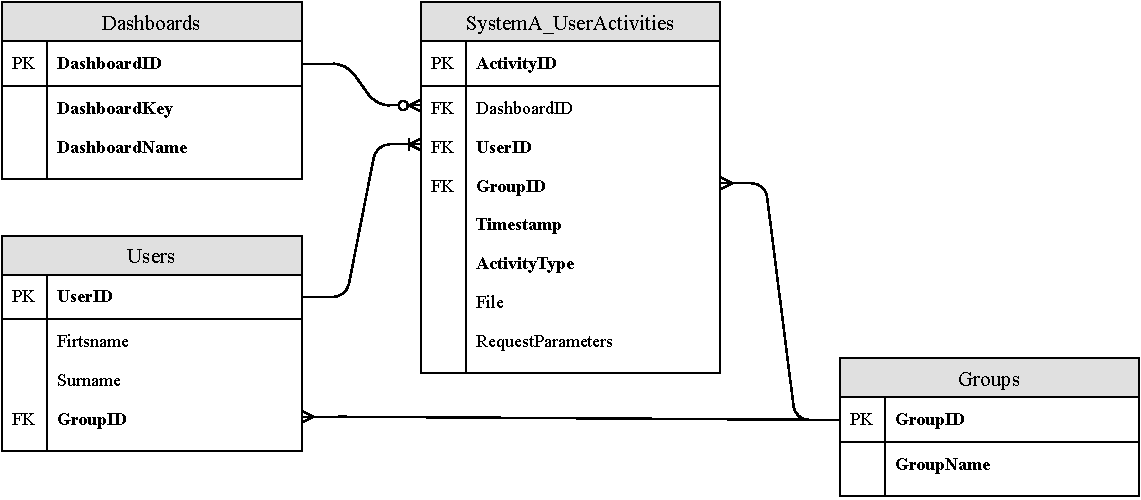
\includegraphics[width=0.9\textwidth]{Chapter2/SystemA_ERD_Basic/SystemA_ERD_Basic.pdf}
	\caption[System A user activity ERD]
	{\textit{System A user activity ERD}}\label{fig:Ch2_SystemA_Basic_ERD}
\end{figure}

\clearpage

In \Cref{fig:CH2_SystemBMetaData} is the metadata JSON for the RequestParameters column in \Cref{tbl:Ch2_System_A_Logging_Points}. This JSON contains certain data parameters important to the event that the user has initiated. This request parameters will need to be specified for each toolbox and dashboard the user events are logged off for System A.

\begin{figure}[!htb]
	\centering
	\begin{lstlisting}[style=json] 
	{
		"Parameter1": 4,
		"Parameter2": "Hello World!",
		"Parameter3": true
		"Parameter4": 40.404
	}
	\end{lstlisting}
	\caption[System A meta data JSON]
	{\textit{System A meta data JSON}}\label{fig:CH2_SystemAMetaData}
\end{figure}

\subsubsection{System A logging mechanism design}
\Cref{sec:SystemA_LoggingPoints} the logging points System A's key logging points need to be captured by a logging mechanism. In \Cref{fig:ch2_systemDesign2} is the design for the System A's logging mechanism to effectively log the user generated event from the PHP software components. The logging mechanism consist of two main functional requirements (\textbf{F/R}) which is the client and server functional requirements.

\begin{figure}[!htb] % An h :here, t: top, b: bottom.
	\centering % cent the figure
	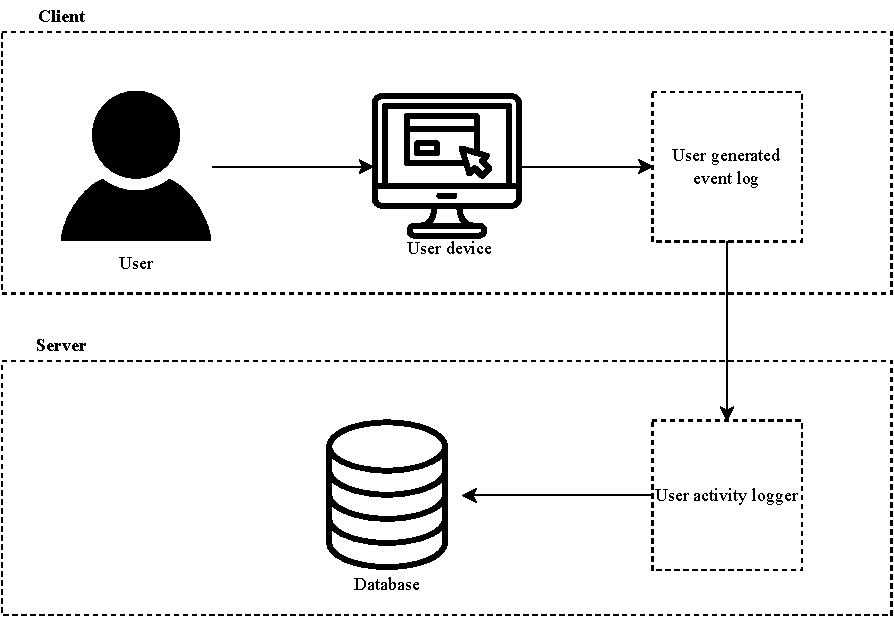
\includegraphics[width=0.9\textwidth]{Chapter2/SystemA_Architecture_Diagram/SystemA_Architecture_Diagram.pdf}
	\caption[System A logging mechanism architecture design]
	{\textit{System A logging mechanism architecture design}}\label{fig:ch2_systemDesign2}
\end{figure}

In the client's functional requirements (F/R 1) the user is the main focus and is the initiator of user activity event logs that take place in System A. The user has a direct interface (I/F 1.1) to the device (F/R 1.2) that is currently browsing System A's websites for specific tasks.\par If the user initiates an activity the request will in most cases either be handled in the dashboard manager of System A or on a defined file where the dashboards software components are. These activities are either captured by the logging mechanisms of \Cref{fig:ch2_Dash_PHP_Flow} or \Cref{fig:ch2_DetailView_Flow} that gets the necessary parameters and defines the type of the user generated event of \Cref{tbl:Ch2_SystemA_EventTypes}. \par The user-generated event (F/R 1.3) is sent to the user activity tracker logger (F/R 2.1) which is the database interaction of the logging mechanism as in \Cref{fig:CH2_SystemA_DB_Interaction_FlowDiagram} to create a log entry in the SQL database of (F/R 2.2).

\subsubsection{Dash user activty type classification}

In \Cref{fig:ch2_Dash_PHP_Flow} is the process of getting the Dash and Report user activity event type for System A. In System A there are certain software components in a dashboard manager file that manages the dashboards according to which the user has selected to view. This dashboard manager file will always execute the needed processes to manage the dashboard upon is the start-up phase.\par When the user sends a request to view a dashboard the requested dashboard's ID send to the dashboard manager. The dashboard manager will attempt to get the dashboard based on the provided dashboard ID. If the request doesn't contain a dashboard ID parameter, any attempt to log the activity will be ended and will be handled with the logging process described in \Cref{fig:ch2_DetailView_Flow}. \par If the dashboard ID parameter does exist and is not an empty or null value it will be added to the activity parameters. The activity parameters consist of some of the parameters needed for \Cref{tbl:Ch2_System_A_Logging_Points} when the event log is eventually saved in the database. \par In System A there are reports generated and some of the events of the report generation will use the dashboard manager's file. These user-generated events can only be traced there and will send an action parameter that is use to initiate the report generation process.\par The action parameters in System A is parameters set in the Post and Get methods. If the action parameter contains report generation value the activity type needs to be set to the Report user activity type otherwise it is set the Dash user activity type. After the additional parameters and activity type parameters are set the ActivityTracker function is called to complete the log and save it in the SQL database as in \Cref{fig:CH2_SystemA_DB_Interaction_FlowDiagram}. 

\begin{figure}[!htb] % An h :here, t: top, b: bottom.
	\centering % cent the figure
	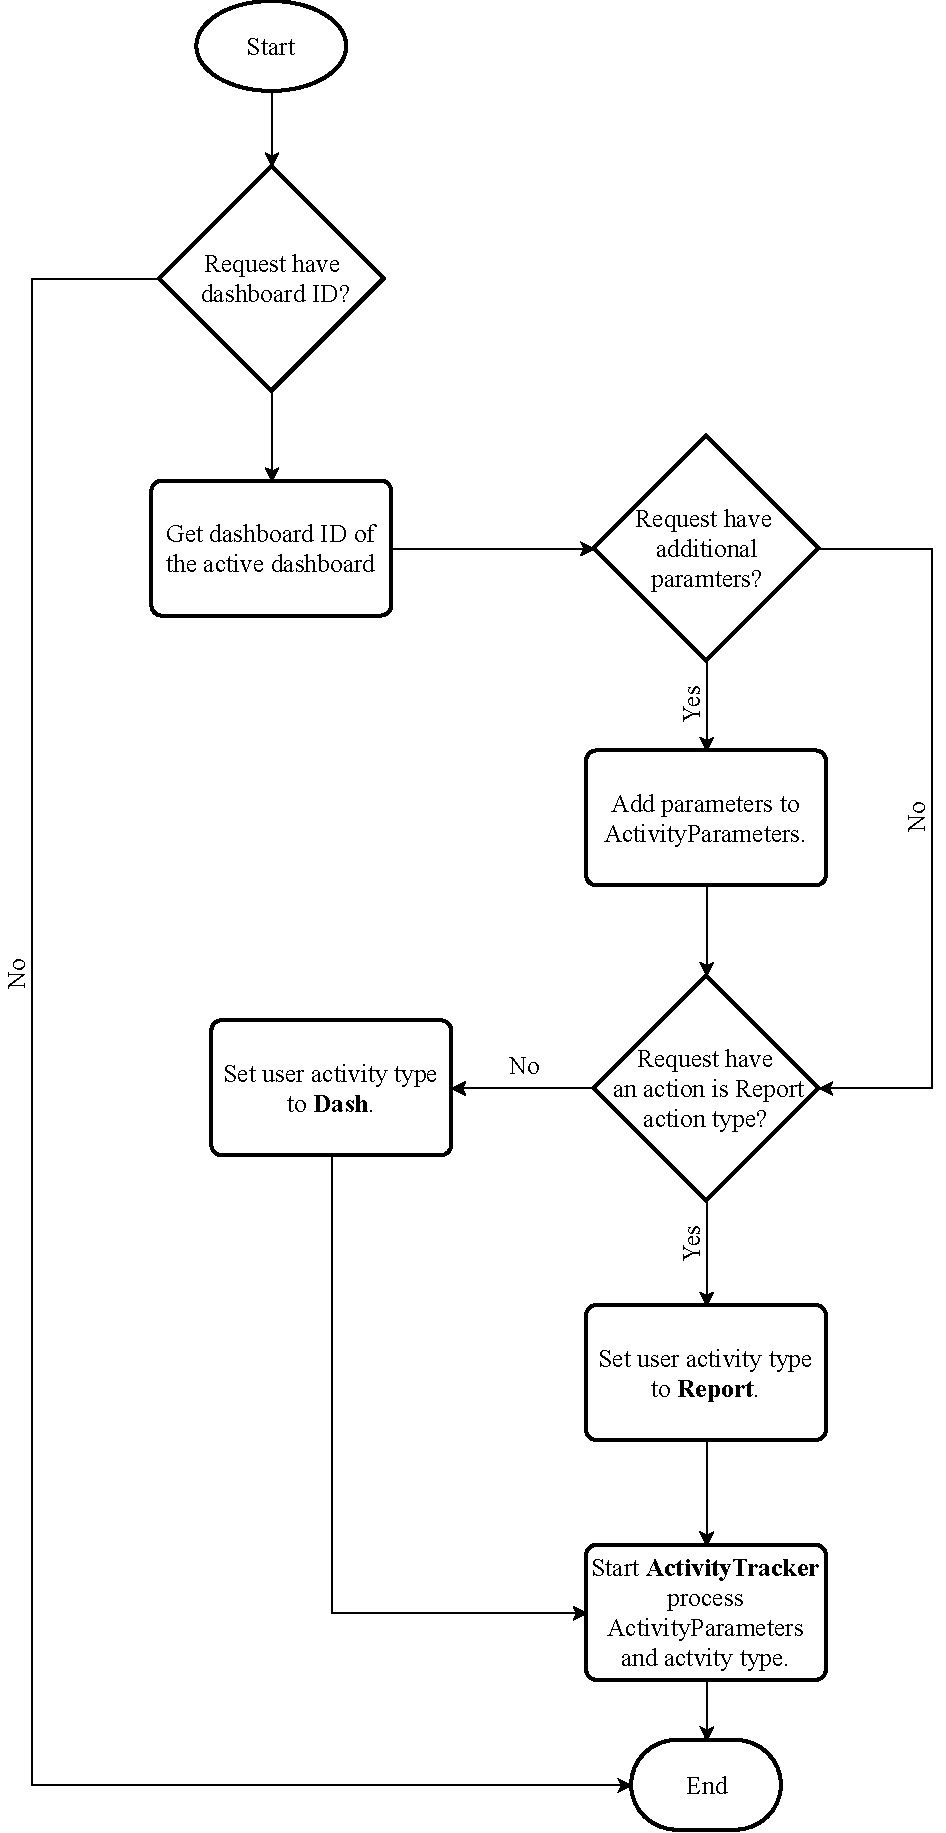
\includegraphics[width=0.7\textwidth]{Chapter2/Dash_PHP_Flow/Dash_PHP_Flow.pdf}
	\caption[User activity logging of Dash and Report event types]
	{\textit{User activity logging process of Dash and Report event types flow diagram}}\label{fig:ch2_Dash_PHP_Flow}
\end{figure}

\clearpage

\subsubsection{User activity logging process of DetailView and Report event types}

In \Cref{fig:ch2_DetailView_Flow} is the process of getting the DetailView and Report user activity event type for System A. This logging process is used in each file that dashboards are created from. In \Cref{fig:ch2_SystemA_Dashboard} multiple dashboards can use the same files with different configuration parameters send with the request, therefore this significantly reduces the needed development to enable the user activity tracking for the dashboards.\par After the user has navigated to their selected dashboard, any user generated request is logged as user activities in System A. These events can be divided into the DetailView and Report event types based on their action parameters that is sent with the request. If the event doesn't have any action parameters, the logging process terminates as this event doesn't count as a valid user activity event.\par If the event does have any action parameters it is checked whether the parameters have report generation value or not. If the event have report action values then the user activity type is set to the Report event type otherwise it is set to DetailView event type.\par There may exist any additional parameters that is send with the request that can be logged. These parameters will vary more than the additional parameters of the Dash events as the Dash events parameters is used to configure the dashboard and not get certain variations activities the user performs on the dashboard.\par If the additional parameters are not null or empty values they are added to the ActivityParameters. With the set ActivityParameters and the defined user activity type the ActivityTracker process of \Cref{fig:CH2_SystemA_DB_Interaction_FlowDiagram} to create a log entry that is saved in the SQL database.

\begin{figure}[!htb] % An h :here, t: top, b: bottom.
	\centering % cent the figure
	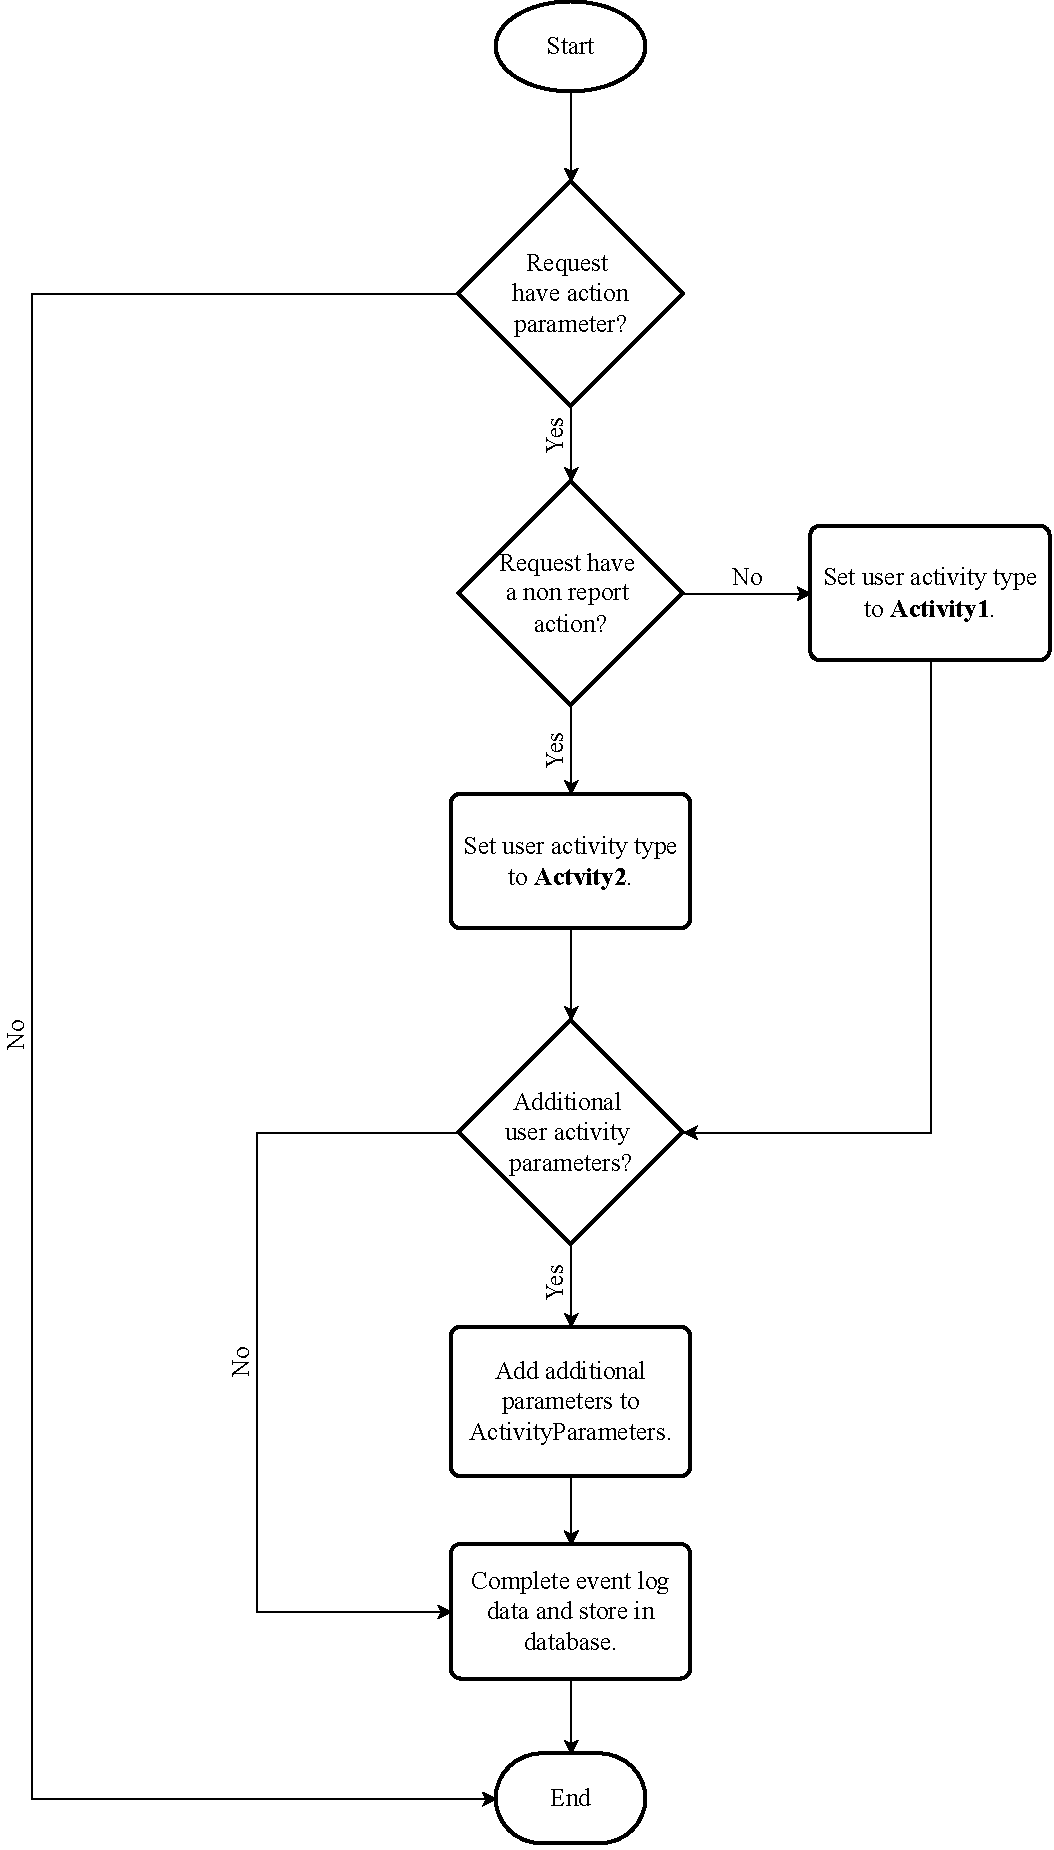
\includegraphics[width=0.75\textwidth]{Chapter2/DetailView_Flow/DetailView_Flow.pdf}
	\caption[User activity logging of DetailView and Report event types]
	{\textit{User activity logging process of DetailView and Report event types flow diagram}}\label{fig:ch2_DetailView_Flow}
\end{figure}

\clearpage

\subsubsection{Database interaction of the logging mechanism}\label{sec:CH2_SystemA_DB_Interaction_FlowDiagram}

In \Cref{fig:ch2_Dash_PHP_Flow,fig:ch2_DetailView_Flow} the user-generated event is captured with additional parameters that may exist with the captured event. The next process in \Cref{fig:CH2_SystemA_DB_Interaction_FlowDiagram} is save the generated user activity log in a database.\par \Cref{fig:CH2_SystemA_DB_Interaction_FlowDiagram} is the process which the logging mechanism will create a log entry by first initialising the SQL database connection. The last parameter needed to complete the requirements of the logging points in \Cref{tbl:Ch2_System_A_Logging_Points} is the user's identification. This is obtained from the user's session that contains the user's ID number that is assigned in the Users table.\par The ActivityParameters from  \Cref{fig:ch2_Dash_PHP_Flow,fig:ch2_DetailView_Flow} are encoded as a JSON string to be saved in the RequestParameters column. After all the parameters are converted to correct format the SQL query created and executed to save the log entry in the SystemA\_UserActivities table of \Cref{fig:Ch2_SystemA_Basic_ERD}.

\begin{figure}[!htb] % An h :here, t: top, b: bottom.
	\centering % cent the figure
	\includegraphics[width=0.5\textwidth]{Chapter2/SystemA_ActivityTracker/SystemA_ActivityTracker.pdf}
	\caption[User activity logging mechanism database interaction]
	{\textit{User activity logging mechanism database interaction}}\label{fig:CH2_SystemA_DB_Interaction_FlowDiagram}
\end{figure}

\clearpage

\subsection{System B}

\subsubsection{System B's logging points}

In \Cref{fig:ch2_Flow_MVC_Architecture} is a diagram of the request flow of a MVC architecture that shows how the user interacts with it. The user will send multiple requests from their own device (client device) via an Internet connection to the server that processes the request. The software system will read and write data from the database source to create a result that send back to the client device for the user. System B is based on this type of architecture to display multiple menus to the user. 

\begin{figure}[!htb] % An h :here, t: top, b: bottom.
	\centering % cent the figure
	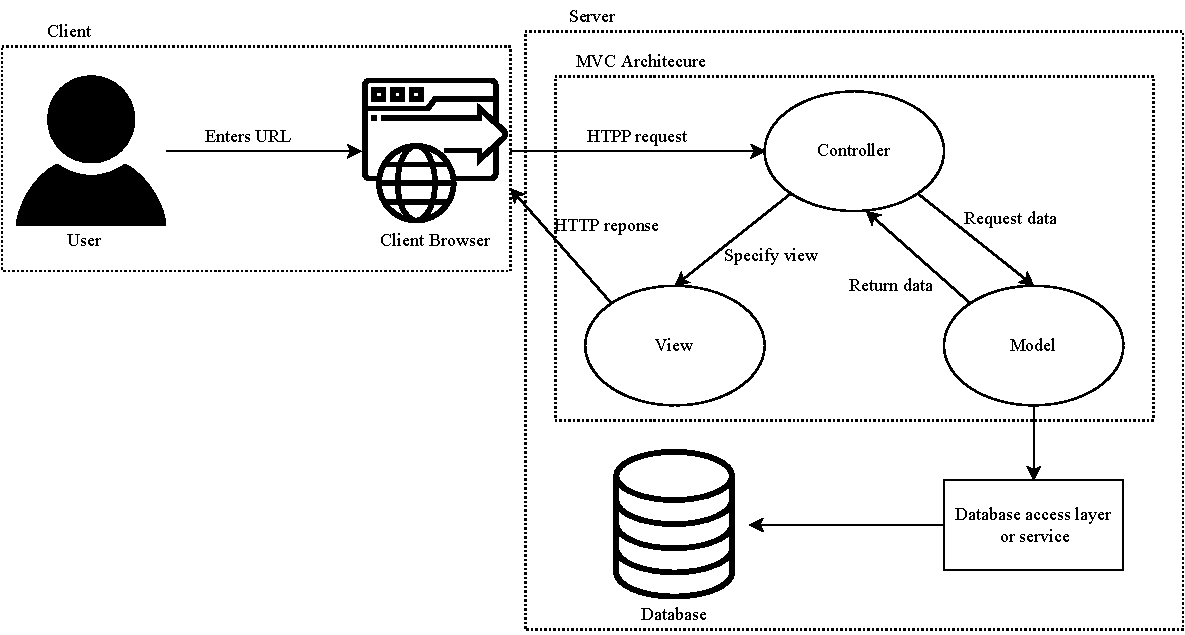
\includegraphics[width=0.95\textwidth]{Chapter2/Flow_MVC_Architecture/Flow_MVC_Architecture.pdf}
	\caption[Request flow in MVC architecture]
	{\textit{Request flow in MVC architecture \cite{Gu2010}}}\label{fig:ch2_Flow_MVC_Architecture}
\end{figure}

In \Cref{sec:SystemA_LoggingPoints} System A mostly relies on the user sessions data to obtain the user-generated event's data, for System B this data can be obtained by the FilterContext class in ASP.NET MVC. The FilterContext provides contains the following information about the request:

\begin{itemize}
	\item \textbf{Absolute URI path:} The string containing the absolute URI path the current controller that is active is part of the FilterContext. This does not reference the controller that handles the request but the controller that user is active on before initiating the request. 
	\item \textbf{Absolute request URL:} The requested URL contains the controller's name and function that process requests. This reference the controller that handles the request but the controller that user is active on before initiating the request. Most of System B's menus are partitioned in separate units which is called Areas in the ASP.NET MVC projects. The area from which the controller is is also part the of this path.
	\item \textbf{Action parameters:} The FilterContext contains action parameters which are the request parameters send with the AJAX request from the client device. These parameters are used in the function that is being called to do certain task within the controller.
\end{itemize}

In System B's session information the user's identification credentials are stored and is used to identify which user initiated the event that is processed.

\clearpage

Using the information from the FilterContext and session of System B the key logging points can be obtained to create \Cref{tbl:CH2_SystemB_LoggingTable} that is saved in SQL database. Each of this logging points can be accessed through a filter action to capture run-time data such as the action parameters that are part of the metadata.

\begin{table}[!htb]
	\centering
	\small
	\caption[System B user activities table]
	{\textit{System B user activities table}}
	\label{tbl:CH2_SystemB_LoggingTable}
	\begin{tabularx}{\textwidth}{|l|l|X|}
		\hline \textbf{Column Name} & \textbf{SQL Data Type} & \textbf{Description} \\
		\hline \textbf{ActivityID} & INT(11) & The activity identification is an incremental number of the event that is logged.\\
		\hline \textbf{Timestamp} & DATETIME & This is the time which the event took place.\\
		\hline \textbf{ActivityType} & ENUM & Each event that the user initiate has an activity type as in \Cref{tbl:Ch2_SystemB_ActivityTypes}. This activity type is dependent if the controller's called method is the index action or based on the HTML element that is part of the meta data. \\
		\hline \textbf{UserID} & INT(4) & Each user has a unique identifier which is a numerical identification number that is foreign key reference to the User table. \\
		\hline \textbf{Area} & VARCHAR(45) & This information is logged to track user activities per Area that represents different software systems that the user can use. \\
		\hline \textbf{Controller} & TEXT & Each event will point back to an controller that process the request. \\
		\hline \textbf{GroupID} & INT(4) & This foreign key reference to the Group table is contract groups identification number. \\
		\hline \textbf{MetaData} & JSON & The meta data of the event contains request parameters, the HTML element from which the request is initiated and other relevant request data of the event. This can also be other meta data is important to get that adds more information about the user's activity using certain controls on System B as in \Cref{fig:CH2_SystemBMetaData}. \\
		\hline
	\end{tabularx}
\end{table}

In \Cref{fig:CH2_SystemBMetaData} the metadata JSON for the user activity log obtained. This JSON contains the request origin of the event from the absolute URI path, HTML element that user used to initiate the event and the request parameters sent with the AJAX request. Some of these JSON parameters can be empty depending on the type of activity.

\begin{figure}[!htb]
	\centering
	\begin{lstlisting}[style=json] 
	{
		"RequestOrigin" : "/Area4/Controller4",
		"RequestElementID" : "Button4",
		"RequestParameters": {
			"Parameter1": 4,
			"Parameter2": "Hello World!",
			"Parameter3": true
			"Parameter4": 40.404
		}
	}
	\end{lstlisting}
	\caption[System B meta data JSON]
	{\textit{System B meta data JSON}}\label{fig:CH2_SystemBMetaData}
\end{figure}

\clearpage

The user activity types in \Cref{tbl:Ch2_SystemB_ActivityTypes} is all of the possible activities the user can generate in System B. The MenuAccessed activity type can be used to track how the user is navigating through the System B just like System A's Dash user activity type. The CustomControls and ElementClickEvents user activity types is the best representation of the system utilisation of System B by the users.

\begin{table}[!htb]
	\centering
	\small
	\caption[System B user activity types]
	{System B user activity types}
	\label{tbl:Ch2_SystemB_ActivityTypes}
	\begin{tabularx}{\textwidth}{|l|X|}
		\hline \textbf{Activity Type} & \textbf{Description} \\
		\hline \textbf{MenuAccessed} & These events are any user activities where the user attempts to access a menu on System B which calls the index method of the menu's controller. In most cases the event request from the client side will be handled by the controller's index function to send back a response of the initial accessing of a specific menu. \\
		\hline \textbf{LogoutAttempt} & Any logout attempt from the user except closing the browser tab or browser. Closing the browser or tab doesn't send any request from the client device back to the server to log that user ended their session. \\
		\hline \textbf{LoginAttempt} & Any user activities on the login page of System B where the user will try enter their credentials to gain access to their user accounts on System B.\\
		\hline \textbf{SessionTracking} & This is any user activities that directly involves extension session due that System B will attempt to logout the user after a hour of inactivity prompting the user to extend their own session.\\
		\hline \textbf{ResetPassword} & Any user activities when the user attempts to reset their password. \\
		\hline \textbf{CustomControls} & System B uses custom controls made the development team, when the user uses these controls it will also initiated an event that can be tracked. \\ 
		\hline \textbf{ElementClickEvents} & Any distinguishable \emph{HTML} element that is clicked by the user that communicates back to the server. These events are ButtonClicked, SelectClicked, ImageClicked, InputClicked, SpanClicked, LabelClicked, ListClicked, HyperLinkClicked, DivClicked, FormInput and GridItem.\\
		\hline
	\end{tabularx}
\end{table}

In \Cref{fig:ch2_SystemB_Basic_ERD} is the ERD of tables directly used for System B. The key logging points of \Cref{tbl:CH2_SystemB_LoggingTable} is used to create the table SystemB\_UserActivities. The data is stored in a SQL database where the Users and Groups tables are. The Users table contains all the information of the users using the System B and the Groups table contains all the mine contract group information. 

\begin{figure}[!htb] % An h :here, t: top, b: bottom.
	\centering % cent the figure
	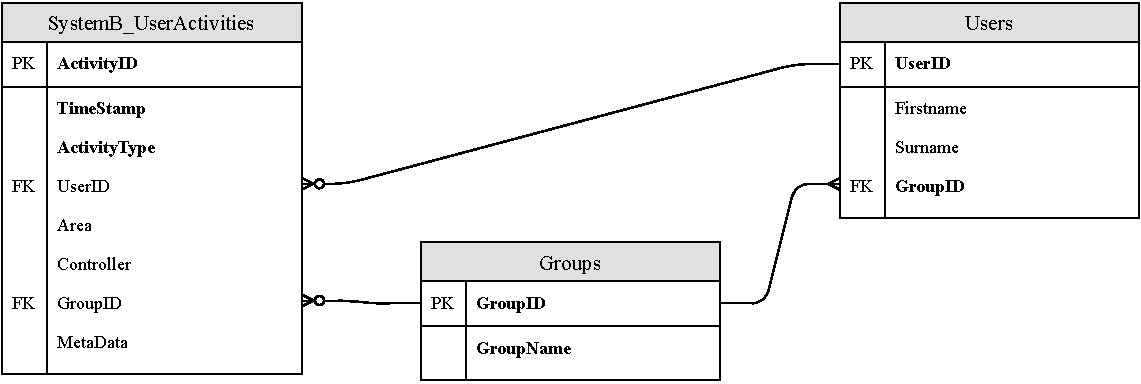
\includegraphics[width=0.99\textwidth]{Chapter2/SystemB_ERD_Basic/SystemB_ERD_Basic.pdf}
	\caption[System B user activity ERD]
	{\textit{System B user activity ERD}}\label{fig:ch2_SystemB_Basic_ERD}
\end{figure}

\clearpage

\begin{figure}[!htb]
	\centering
	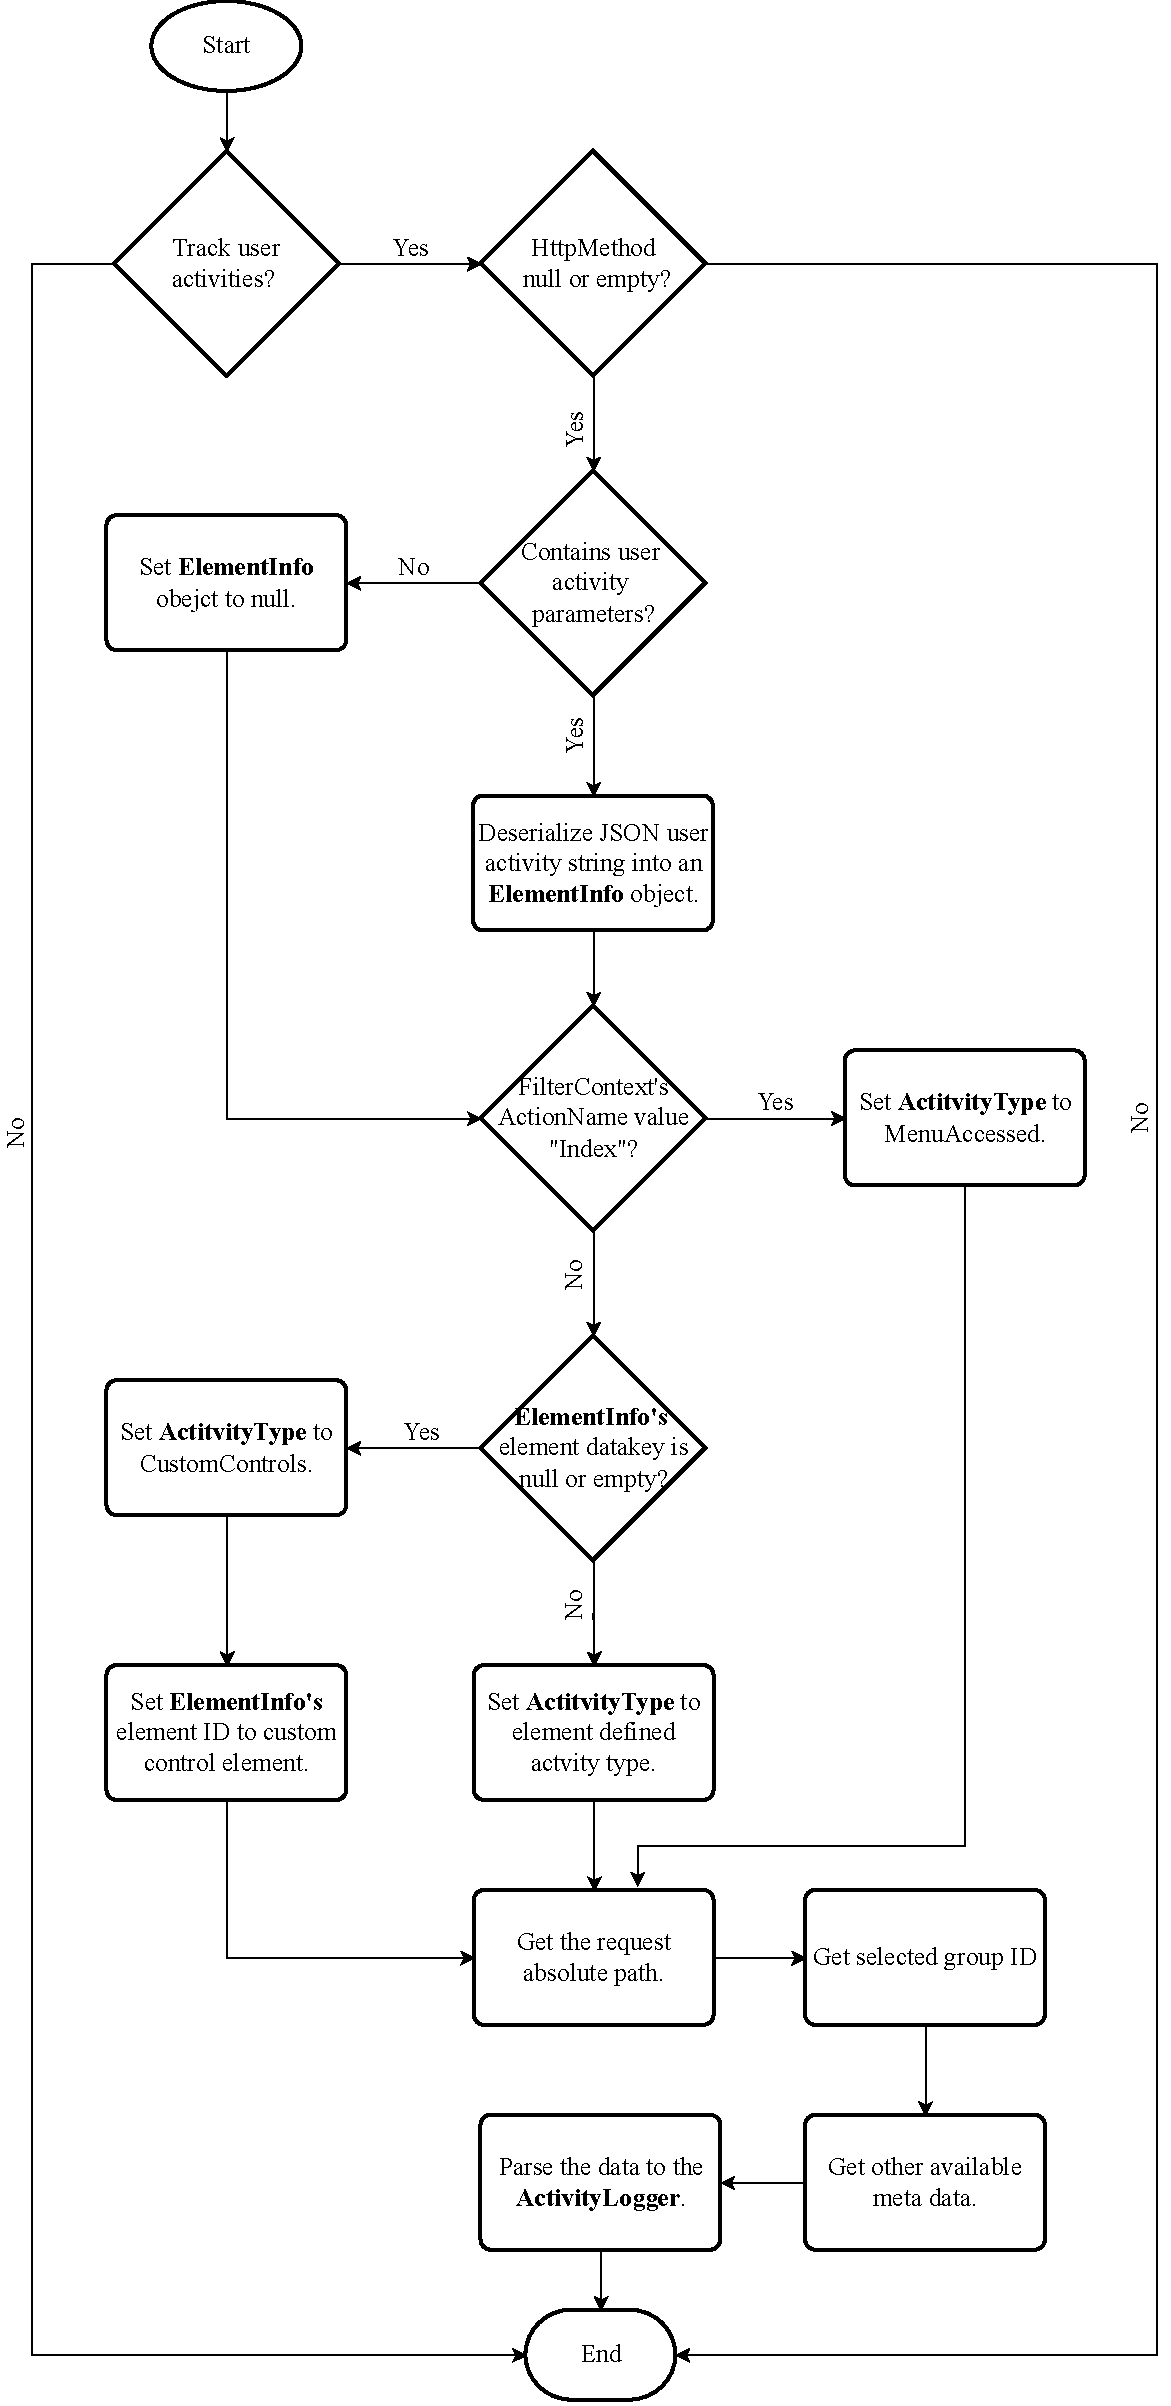
\includegraphics[width=0.7\textwidth]{Chapter2/SystemB_FilterContext/SystemB_FilterContext.pdf}
	\caption[System B event classification]
	{\textit{System B event classification flow diagram}}\label{fig:CH2_SystemB_FilterContext}
\end{figure}

\clearpage

\section{System utilisation analysis}

\section{Integration}
In this section, the integration of the utilisation analysis and logging mechanism will be discussed.

\section{Conclusion}
Conclude the chapter about the development of the logging mechanism and utilisation analysis.

Most Web applications will make of use JavaScript to control the content of the page that is being displayed to the user. The primary method would be making use of an \textit{AJAX request} to communicate with the server to fulfil the user's action.\par The \textit{AJAX request} has some key features that will enable the logging points discussed in \Cref{sec:ch2_loggingPoints} to capture some logging attributes and classify the event as a user-based activity. \par The \texttt{beforeSend} setting of the \textit{AJAX request} enables tracking in real-time for the HTML element id and its HTML tag or other possible log attributes that need to be added to the request for the log point to capture it. The captured HTML element id, HTML tag and some other parameters can be added as a custom request header that will be sent to the server.

\begin{lstlisting}[caption={\textit{AJAX request example \cite{API.jQuery2022}}}, label={fig:ch2_ajaxBeforesend}]  
	$.ajax({
		url: "https://fiddle.jshell.net/favicon.png",
		beforeSend: function (xhr) {
			xhr.overrideMimeType("text/plain; charset=x-user-defined");
		}
	}).done(function (data) {
		if (console && console.log) {
			console.log("Sample of data:", data.slice(0, 100));
		}
	});
\end{lstlisting}

\section{Logging mechanism}

\subsection{Obtaining the element of user-based event}\label{sec:ch2_ElementObtaining}
In \Cref{sec:ch2_webApplicationArchitecture} the user-based activity event will be use a \textit{HTTP request} to send to the server when the user interacted with an \textit{HTML element}. For the functional requirements activity type (F/R 1.5.3) and metadata (F/R 1.5.6) in \Cref{tbl:ch2_keyLoggingAttributes} the \textit{HTML element} needs to be obtained to get the element's tag and identification text. This can be difficult to obtain due to \textit{bubbling}\footnote{\textbf{Bubbling} is when an event happens on an element, it first runs the handlers on it, then on its parent, then up on other ancestors. \cite{EventBubbling}.} that may occur when searching for the element that the user specifically interacted with.\par In \Cref{fig:ch2_event_bubbling} is the event propagation example of a child element that has been clicked on which executes a DOM event. The event propagation consists of three phases~\cite{EventBubbling}:

\begin{itemize}
	\item \textit{Capturing phase:} The event propagates downwards to the targeted element that the user interacted with.
	\item \textit{Target phase:} The event reaches the targeted element to execute the DOM event.
	\item \textit{Bubbling phase:} The event bubbles up from the targeted element
\end{itemize}

\begin{figure}[!htb] % An h :here, t: top, b: bottom.
	\centering % cent the figure
	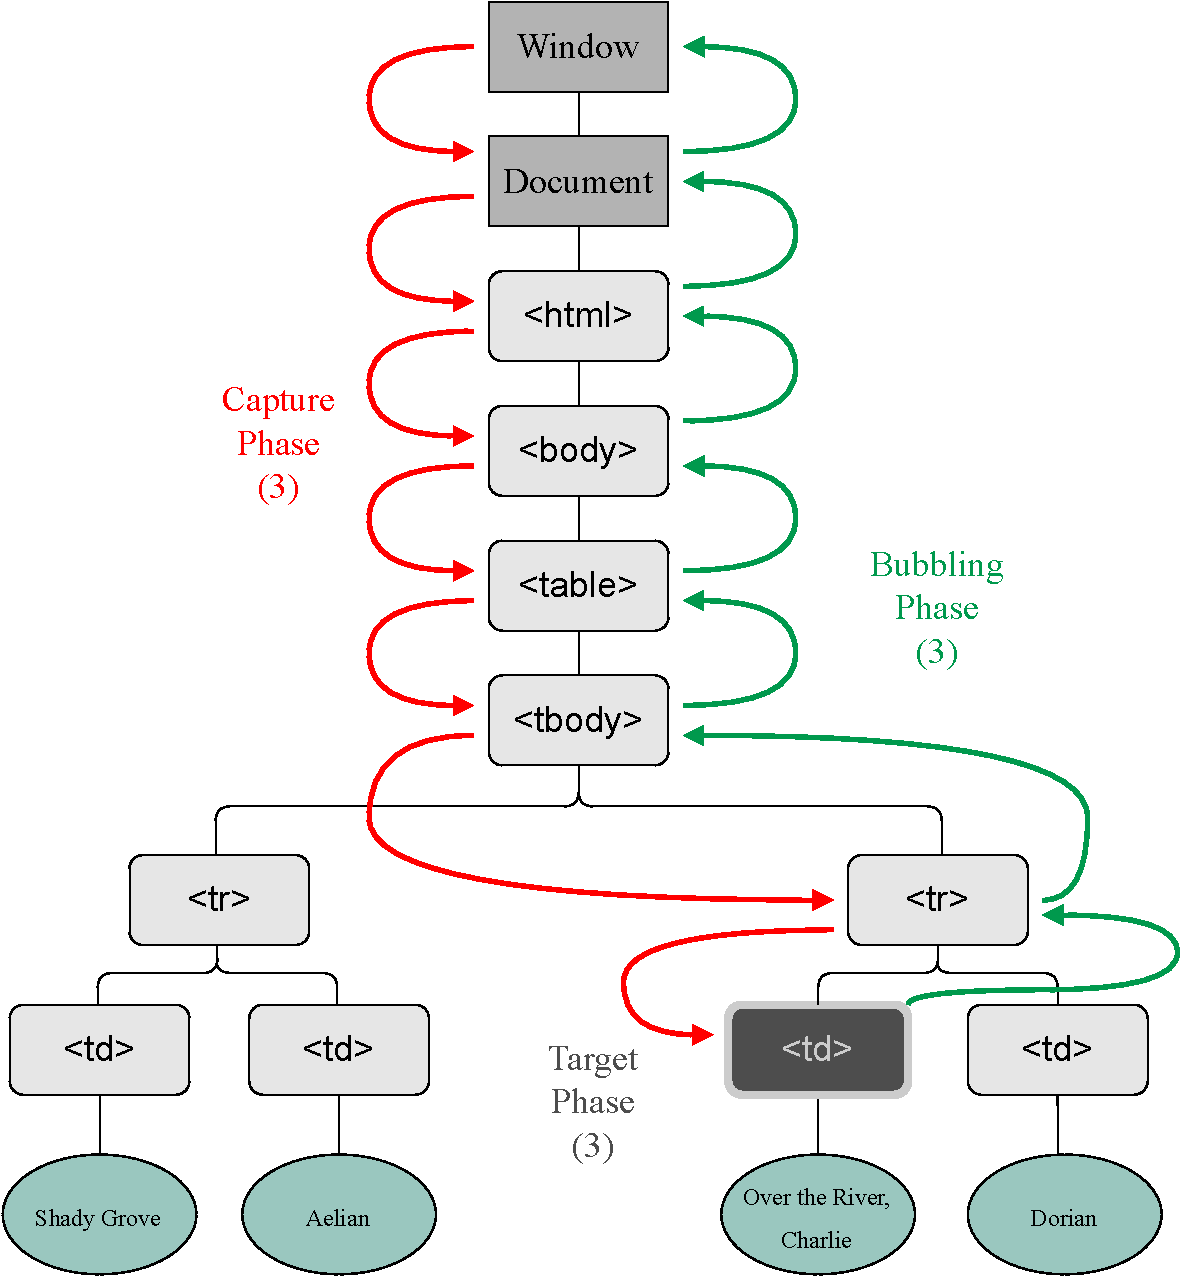
\includegraphics[width=0.6\textwidth]{Chapter2/event_bubbling/event_bubbling.pdf}
	\caption[JavaScript event propagation]
	{\textit{JavaScript event propagation~\cite{EventBubbling}}}\label{fig:ch2_event_bubbling}
\end{figure}

Capturing the targeted element may be difficult as some Web pages may have more complex HTML where the event propagation may sometimes not obtain the correct element information which the user interacted with. Another DOM event may have started during the initial element's event, therefore it is more accurate to obtain the targeted element by obtaining the last known element the user hovered over on the user interface.\par In \Cref{fig:ch2_element_event_capturing} is the flow diagram to capture the element user interacted with for the user-based activity log. This code segment will be initiated during the \texttt{beforeSend} operation of the \textit{AJAX request} to filter HTML elements by predefined allowed elements to use. Filtering the element tag names ensures that unwanted more complex elements or more basic elements that are not expected to be the initiator of the event will be used. \par If the Web location already changed or no element exists, the contents of the page might have already changed during the event propagation. The last known element that the user hovered on must be used as most likely might have been the element that the user interacted with. This will ensure there is always an element that has been detected and parsed with the request header in most UI changes.

\clearpage

\begin{figure}[!htb] % An h :here, t: top, b: bottom.
	\centering % cent the figure
	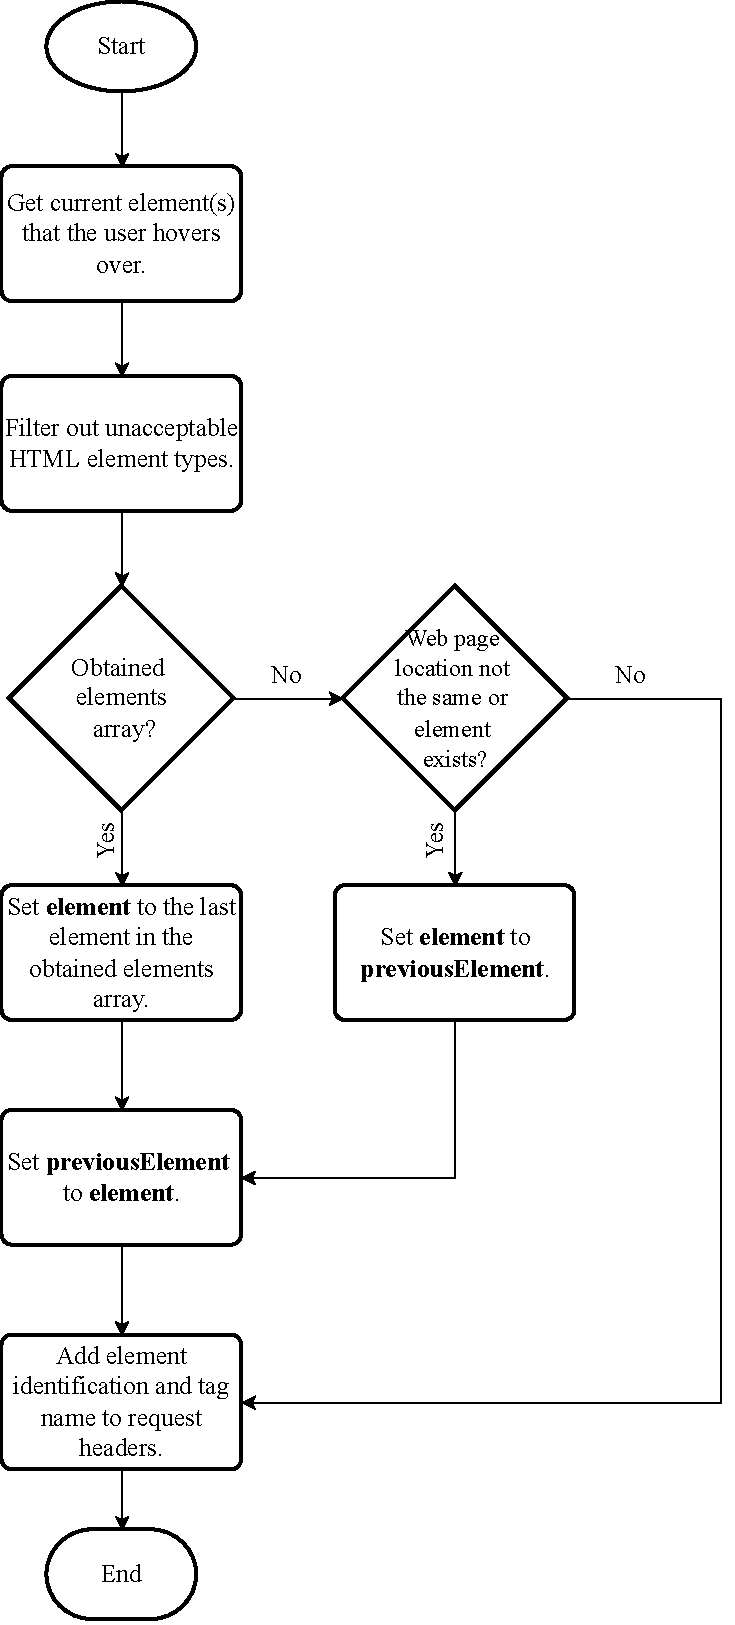
\includegraphics[width=0.5\textwidth]{Chapter2/element_capturing/element_capturing.pdf}
	\caption[HTML element capturing flow diagram]
	{\textit{HTML element capturing flow diagram}}\label{fig:ch2_element_event_capturing}
\end{figure}

\section{Utilisation analysis}


\section{Verification}\label{sec:ch3_verification}
Using the functional requirements defined in \Cref{sec:ch2_loggingMechanism,ch2:sec_system_utilisation_analysis} the system can be verified that it satisfies the system requirements in \Cref{tbl:ch2_verification}.

\begin{table}[!htb]
	\centering
	\caption[System requirements for verification]
	{\textit{System requirements for verification}}
	\label{tbl:ch2_verification}
	\begin{tabularx}{\textwidth}{|X|X|c|}
		\hline \textbf{Requirement} & \textbf{Methodology reference} & \textbf{Satisfied} \\
		\hline \textbf{User activity types} &  & \cmark \\
		\hline \textbf{Log attributes} & & \cmark \\
		\hline \textbf{Logging points} &  & \cmark \\
		\hline \textbf{Log extraction and visualisation} &  & \cmark \\
		\hline \textbf{System utilisation analysis} &  & \cmark \\
		\hline
	\end{tabularx}
\end{table}

\section{Conclusion}

 
%%@@@@@@@@@@@@@@@@@@@@@@@@@@@@@@@@@@@@@@@@@@@@@@@@@@@@@@@@@@@@@@@@@@@@@@@@@@@@@@@@@@@@@@@@@@@@@@@@@@@
%@@        Chapter 6: Conclusion                                                                  @@
%@@@@@@@@@@@@@@@@@@@@@@@@@@@@@@@@@@@@@@@@@@@@@@@@@@@@@@@@@@@@@@@@@@@@@@@@@@@@@@@@@@@@@@@@@@@@@@@@@@@

\chapter{Conclusion}
\label{chap:6}
\ChapterPageStuff{6}

%ooooooooooooooooooooooooooooooooooooooooooooooooooooooooooooooooooooooooooooooooooooooooooooooooooo

\section{Bla bla}

% ------- Bibliography -------
\bibliographystyle{IEEEtran}
\cleardoublepage
\phantomsection
\fancyhead[R]{References}
\addcontentsline{toc}{chapter}{References}
\renewcommand{\bibname}{References}
\bibliography{src/lib/library}

% ------- Appendices -------    
\cleardoublepage
\appendix

\chapter{Logging practice in software engineering}\label{apx:loggingPractice}
Providing a guide for software engineers and developers to implement a suitable logging implementation in their software systems has to prove to be a vital tool in both industrial use and progress of academia \cite{Rong2018a}. Guoping Rong et al.~made a study to review these logging practices published papers to improve the performance and efficiency of logging implementation. From his study he made selection criteria to include (as in \Cref{tbl:CH1_RongIncSelectionCriteria}) and exclude (as in \Cref{tbl:CH1_RongExlSelectionCriteria}) academic papers about logging practices \cite{Rong2018a,Rong2018}.\par The Rong's selection criteria obtained numerous research papers of logging practices applied in the industry by either creating a new logging mechanism or optimising existing logging mechanisms. By reviewing 41 identified papers he found that many practitioners and researchers recognise the importance of logging practice in software engineering. There is a lack of guidance to provide software engineers or developers to create or improve their efficient logging mechanisms \cite{Rong2018a,Zhu2015}. 

\begin{table}[!htb]
	\centering
	\caption[G. Rong's inclusion selection criteria]
	{\textit{G. Rong's inclusion selection criteria \cite{Rong2018a}}}
	\label{tbl:CH1_RongIncSelectionCriteria}
	\begin{tabularx}{\textwidth}{|c|X|}
		\hline \textbf{Identification} & \textbf{Criteria} \\
		\hline I1. & Publications that investigate the methodology for logging practice. \\
		\hline I2. & Publications that investigate the tools, frameworks, systems which support logging practice. \\
		\hline I3. & Publications that propose a standard for logging practice.\\
		\hline I4. & Publications that are peer-reviewed (conference paper, journal article). \\
		\hline I5. & Publications that are primary studies on logging practice. \\
		\hline
	\end{tabularx}
\end{table}

\begin{table}[!htb]
	\centering
	\caption[G. Rong's exclusion selection criteria]
	{\textit{G. Rong's exclusion selection criteria \cite{Rong2018a}}}
	\label{tbl:CH1_RongExlSelectionCriteria}
	\begin{tabularx}{\textwidth}{|c|X|}
		\hline \textbf{Identification} & \textbf{Criteria} \\
		\hline E1. & Publications that investigate log analysis. \\
		\hline E2. & Publications that investigate the usage of logs. \\
		\hline E3. & Publications that investigate the technologies on logging user behaviours. \\
		\hline E4. & Publications that are not written in English. \\
		\hline E5. & Additionally, short papers, demo or industry publications are excluded. \\
		\hline
	\end{tabularx}
\end{table}

\clearpage

In \Cref{fig:PushblisedPapers} shows the distribution of the 41 published papers obtained for Rong's research relating to logging practices. Event logging has an increasingly important role in modern software systems, therefore the research focus on logging practices in software engineering have been on a rise between 1990 and 2017.

\begin{figure}[!htb] % An h :here, t: top, b: bottom.
	\centering % cent the figure
	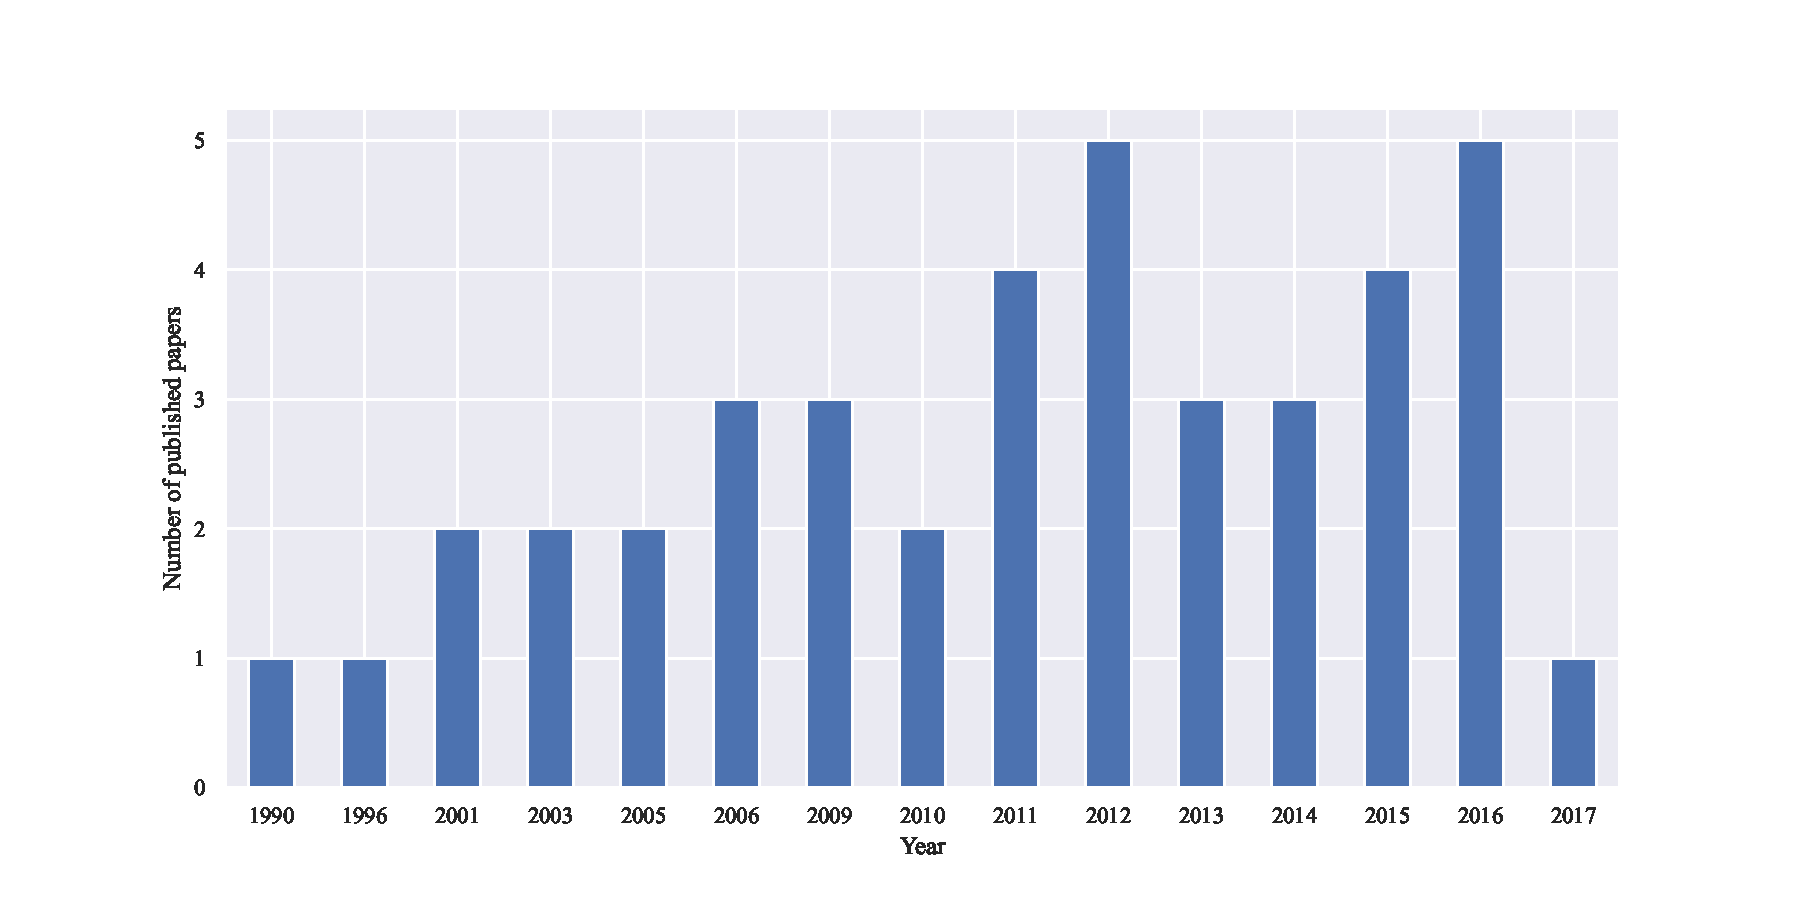
\includegraphics[width=0.95\textwidth]{Chapter1/Ronga2018.pdf}
	\caption[The distribution of the papers’ published years]
	{\textit{The distribution of the papers’ published years \cite{Rong2018a}}} \label{fig:PushblisedPapers}
\end{figure} 


\end{onehalfspace}

\end{document}
